% TEMPLATE for Usenix papers, specifically to meet requirements of
%  USENIX '05
% originally a template for producing IEEE-format articles using LaTeX.
%   written by Matthew Ward, CS Department, Worcester Polytechnic Institute.
% adapted by David Beazley for his excellent SWIG paper in Proceedings,
%   Tcl 96
% turned into a smartass generic template by De Clarke, with thanks to
%   both the above pioneers
% use at your own risk.  Complaints to /dev/null.
% make it two column with no page numbering, default is 10 point

% Munged by Fred Douglis <douglis@research.att.com> 10/97 to separate
% the .sty file from the LaTeX source template, so that people can
% more easily include the .sty file into an existing document.  Also
% changed to more closely follow the style guidelines as represented
% by the Word sample file. 

% Note that since 2010, USENIX does not require endnotes. If you want
% foot of page notes, don't include the endnotes package in the 
% usepackage command, below.

% This version uses the latex2e styles, not the very ancient 2.09 stuff.
\documentclass[letterpaper,twocolumn,10pt]{article}
\usepackage{usenix,epsfig,endnotes}

\usepackage{times}
\usepackage{CJKutf8}
\usepackage{mathrsfs}
\usepackage{textcomp}
\usepackage{verbatim}
\usepackage{amsmath}
\usepackage{amsfonts}
\usepackage{xspace}
\usepackage{xcolor}
\usepackage{url}
\usepackage{balance}
\usepackage{booktabs}
\usepackage{multirow}
\usepackage{rotating}
\usepackage{fancyvrb}
\usepackage{lastpage}
\usepackage{alltt}
\usepackage{etoolbox}
\usepackage{cleveref} % After hyperref, listings
\usepackage{fancyhdr}
\usepackage{listings}

\usepackage{caption}
\usepackage{subcaption}

\usepackage{tikz}
\usetikzlibrary{shapes,snakes}


\usepackage{amsmath}
\usepackage{amssymb}
\usepackage{wasysym}

%The given symbol or text (\text{mytext}) in a circle
%To be used always in math mode
\newcommand{\circlesign}[1]{ 
    \mathbin{
        \mathchoice
        {\buildcirclesign{\displaystyle}{#1}}
        {\buildcirclesign{\textstyle}{#1}}
        {\buildcirclesign{\scriptstyle}{#1}}
        {\buildcirclesign{\scriptscriptstyle}{#1}}
    } 
}


\newcommand\buildcirclesign[2]{%
    \begin{tikzpicture}[baseline=(X.base), inner sep=0, outer sep=0]
    \node[draw,circle] (X)  {\ensuremath{#1 #2}};
    \end{tikzpicture}%
}

\definecolor{lbcolor}{rgb}{0.9,0.9,0.9}
\lstset{
    tabsize=2,    
    language=C,
    basicstyle=\footnotesize\ttfamily,
    upquote=true,
    aboveskip={1.5\baselineskip},
    columns=fixed,
    extendedchars=false,
    showtabs=false,
    showspaces=false,
    showstringspaces=false,
    identifierstyle=\ttfamily,
    keywordstyle=\color[rgb]{0,0,1},
    commentstyle=\color[rgb]{0.026,0.112,0.095},
    stringstyle=\color[rgb]{0.627,0.126,0.941},
    numberstyle=\color[rgb]{0.205, 0.142, 0.73},
}


\usepackage{macro}
\newenvironment{CompactItemize}{\begin{itemize}}{\end{itemize}}
\def\code#1{{\texttt{#1}}}


\usepackage{colorhist}
 
\usepackage{minted}


\begin{document}

%don't want date printed
\date{}

%make title bold and 14 pt font (Latex default is non-bold, 16 pt)
\title{\Large \bf A Lightweight Log-based Deferred Update for Linux Kernel
Scalability}

%for single author (just remove % characters)
%\author{
%{\rm Your N.\ Here}\\
%Your Institution
%\and
%{\rm Second Name}\\
% \and
% {\rm Name}\\
%Name Institution
%} % end author

\maketitle

%한글 버전으로 출력 하고 싶으면, korture를 Enable 해주시고, korefalse를 주석 처리 해주세요.
\newif\ifkor
\kortrue 
%\korfalse

% Use the following at camera-ready time to suppress page numbers.
% Comment it out when you first submit the paper for review.
\thispagestyle{empty}

\subsection*{Abstract}
We propose a novel light weight concurrent update method, \deferu, 
to improve performance scalability for Linux kernel on many-core systems
through eliminating lock contentions for update-heavy global data structures
during process spawning and optimizing update logs. 
The proposed \deferu is implemented into Linux kernel 4.5 and evaluated 
using representative benchmark programs. 
Our evaluation reveals that the Linux kernel with \deferu shows performance
improvement by ranging from Xx through Xx on a 120 core system.

\ifkor
\begin{CJK}{UTF8}{}\CJKfamily{mj}
\fi
\section{Introduction} \label{sec:introduction}

%$$$$$$$$$$$$$$$$$$$$$$$$$$$$$$$$$$$$$$$$$$$$$$$$$$$$$$$$$$$$$$$$$$$$$$$$$$$$$$$$
%$$$$$$$$$$$$$$$$$$$$$$$$$$$$$$$$$$$$$$$$$$$$$$$$$$$$$$$$$$$$$$$$$$$$$$$$$$$$$$$$
%Background
%$$$$$$$$$$$$$$$$$$$$$$$$$$$$$$$$$$$$$$$$$$$$$$$$$$$$$$$$$$$$$$$$$$$$$$$$$$$$$$$$
\ifkor
최근 코어수가 증가하고 있다. 따라서 멀티코어에서 매니코어 환경으로 바뀌고 있다. 
이러한 매니코어 환경에서 리눅스 커널의 확장성에는 문제가 있다[][][]. 
확장성 문제 중 하나는 락 경합 때문에 발생하는 직렬화 문제이다[][].
여러 락 때문에 발생하는 직렬화 문제 중 하나가 update operation이기 때문에 문제가 발생한다[][].
그 이유는 update operation는 여러 thread가 동시에 수행되지 못하기 때문이다.
예를 들어, 리눅스 커널의 프로세스간 공유하는 자료구조인 reverse page maps은 update rate가 높은 구조로 되어
있다[][]. 
따라서 리눅스 커널은 reverse page mapping에 대한 update lock에 때문에 serialize 되어 새로운 프로세스를
생성 하는 과정에서 scalability 문제가 있다[][].
\else

\fi


%$$$$$$$$$$$$$$$$$$$$$$$$$$$$$$$$$$$$$$$$$$$$$$$$$$$$$$$$$$$$$$$$$$$$$$$$$$$$$$$$
%$$$$$$$$$$$$$$$$$$$$$$$$$$$$$$$$$$$$$$$$$$$$$$$$$$$$$$$$$$$$$$$$$$$$$$$$$$$$$$$$
%Problem
%$$$$$$$$$$$$$$$$$$$$$$$$$$$$$$$$$$$$$$$$$$$$$$$$$$$$$$$$$$$$$$$$$$$$$$$$$$$$$$$$
\ifkor
이처럼 update serialization 문제를 해결하기 위해 여러 concurrent updates 방법[][][][][][] 들이 연구되고 있다. 
이러한 concurrent updates 방법들은 워크로드 특성인 update ratio에 따라 많은 성능 차이를 보인다[][].
이 중 리눅스 커널의 reverse page mapping과 같이 high update ratio를 가진 update-heavy한 data
structure일 경우에는, update lock 경합 때문에 발생하는 scalability 문제를 해결하기 위한 여러 방법이 있다.
그 중 하나는 cache coherence traffic을 줄인 log-based 알고리즘[][][]을 사용하는 것이다.
Log-based 알고리즘은 lock을 피하기 위해 update가 발생하면, data structure의 update
operation(insert or remove)을 argument와 함께 저장하고, 주기적 또는 read operation을 수행하기 전에
applies the updates in all the logs to the data structure, so reader can read
up to date data structure. 이것은 마치 CoW(Copy On Write)와 유사한 결과를 얻는다. 

S. Boyd-Wickizer et al. 는 synchronized timestamp counters 기반의 per-core log를 활용하여
update heavy한 자료구조에서의 concurrent updates 문제를 해결하였다.
Synchronized timestamp counters 기반의 per-core log를 활용한 concurrent updates 방법은
update 부분만 고려했을 때, conflict free이므로 굉장히 높은 scalability를 가질 수 있다[]. 
하지만 per-core 기반의 synchronized timestamp counters를 사용한 방법은 결국 timestamp
ordering and merging 작업을 야기한다. 
만약 코어 수가 늘어 날 경우, resolving logs(merging or absorbing) may require
additional sequential processing, which can limit scalalbility and
performance.
Furthermore, because limiting the per-core memory size, OpLog does not work
well for all data structures.
%(OpLog는 각각의 per-core메모리에 저장된 로그의 오브젝트를 해쉬 테이블을 통해 구별한다.)
%(OpLog distinguishs each log's object saving the per-core memory through(via)
% hash table).
\else

\fi



%$$$$$$$$$$$$$$$$$$$$$$$$$$$$$$$$$$$$$$$$$$$$$$$$$$$$$$$$$$$$$$$$$$$$$$$$$$$$$$$$
%$$$$$$$$$$$$$$$$$$$$$$$$$$$$$$$$$$$$$$$$$$$$$$$$$$$$$$$$$$$$$$$$$$$$$$$$$$$$$$$$
%Method
%$$$$$$$$$$$$$$$$$$$$$$$$$$$$$$$$$$$$$$$$$$$$$$$$$$$$$$$$$$$$$$$$$$$$$$$$$$$$$$$$
%
\ifkor
본 논문은 high update rate를 가진 data structure를 위한 새로운 방법인 LDU를 제안한다. 
LDU는 synchronized timestamp counters를 이용함에 따라 생기는 ordering or merging overhead와
workload에 따른 interfaces dependency가 있는 문제를 줄이기 위해, 조금 더 simple하고
lightweight한 방법을 사용하였다.
즉 우리는 update-heavy한 data structure를 위한 새로운 concurrent updates 방법을 제안한다. 
LDU의 철학은 FC 또는 OpLog와 같이 분산 시스템에서 사용하는 log기반의 concurrent updates 방식과 최소한의
shared-memory system의 hardware-based synchronization 기법(예를 들어, compare and
swap, test and set) 이용하여 이 문제를 해결 하였다.
LDU는 per-core 방식이기 때문에 발생하는 interfaces dependency가 있는 문제를 해결하기 위해, log 저장을
global queue를 사용하는 방식인 GLDU와 per-core에 log를 저장하여 global header의 cache
coherece traffic을 줄인 PLDU로 개발하였으며 이것은 서로간 장단점을 가지고 있다.
또한 update-side absorbing과 reuse garbage등 2가지 optimization 기술을 사용하여 삭제 가능한
operation log를 지우고 재활용하는 방법으로 성능 최적화를 수행하였다.

이처럼 synchronized timestamp counters를 제거함과 동시에, cache communication bottleneck 줄인
LDU는 전형적인 log-based 알고리즘의 장점을 모두 가진다.
첫째로, update가 수행하는 시점 즉 로그를 저장하는 순간에는 lock이 필요가 없다. 
따라서 lock 없이 update를 concurrent하게 수행할 수 있다
둘째로, 저장된 update operation log를 corse-grain lock과 함께 하나의 코어에서 수행하기 때문에,
cache 효율성이 높아진다[FC].
셋째로, 기존 여러 데이터 structure에 쉽게 적용할 수 있는 장점이 있다.
마지막으로 저장된 log를 수행하지 전에 optimization 방법을 사용하여 log의 수를 줄 인다.
\else

\fi

%$$$$$$$$$$$$$$$$$$$$$$$$$$$$$$$$$$$$$$$$$$$$$$$$$$$$$$$$$$$$$$$$$$$$$$$$$$$$$$$$
%$$$$$$$$$$$$$$$$$$$$$$$$$$$$$$$$$$$$$$$$$$$$$$$$$$$$$$$$$$$$$$$$$$$$$$$$$$$$$$$$
%Result
%$$$$$$$$$$$$$$$$$$$$$$$$$$$$$$$$$$$$$$$$$$$$$$$$$$$$$$$$$$$$$$$$$$$$$$$$$$$$$$$$

\ifkor
우리는 위와 같은 장점을 가지는 LDU를 리눅스 커널의 fork scalability 문제를 야기시키는 2가지 reverse page
mapping(anonymous pape mapping[], file page mapping[])에 적용하였다.
또한 We implemented the LDU in a Linux 4.5.rc4 with elemination of lock. 
We evaluated the performance and scalability using a fork-intensive workload-
AIM7[], Exim from MOSBENCH[], lmbench[]-our design improves throughput and
execution time on 120 core by 1.7x, 1.6x, 2.2x respectively, relative to stock Linux.
  
\else

\fi




%$$$$$$$$$$$$$$$$$$$$$$$$$$$$$$$$$$$$$$$$$$$$$$$$$$$$$$$$$$$$$$$$$$$$$$$$$$$$$$$$
%$$$$$$$$$$$$$$$$$$$$$$$$$$$$$$$$$$$$$$$$$$$$$$$$$$$$$$$$$$$$$$$$$$$$$$$$$$$$$$$$
%Contribution 정리
%$$$$$$$$$$$$$$$$$$$$$$$$$$$$$$$$$$$$$$$$$$$$$$$$$$$$$$$$$$$$$$$$$$$$$$$$$$$$$$$$
\ifkor
\noindent
\textbf{Contributions.} This paper makes the following contributions:
\begin{itemize}
\item 우리는 새로운 log-based concurrnet updates 방법인 LDU를 개발하였다. 
LDU는 synchronized timestamp counters를 이용함에 따라 생기는 ordering or merging overhead와
workload에 따른 interfaces dependency가 있는 문제를 줄이기 위해, 조금 더 simple하고
lightweight한 방법과 update-side absorbing과 reuse garbage의 optimization을
사용하여 log-based concurrent updates를 구현하였다.
\item 우리는 LDU을 practical한 manycore system인 intel xeon 120코어 위에 동작하는 리눅스 커널에
적용하여, fork scalability 문제를 해결하였다. 
Fork 관련 벤치마크 성능은 워크로드 특성에 따라 1.6x부터 2.2x까지 개선되었다.
\end{itemize}
\else

\fi





%$$$$$$$$$$$$$$$$$$$$$$$$$$$$$$$$$$$$$$$$$$$$$$$$$$$$$$$$$$$$$$$$$$$$$$$$$$$$$$$$
%$$$$$$$$$$$$$$$$$$$$$$$$$$$$$$$$$$$$$$$$$$$$$$$$$$$$$$$$$$$$$$$$$$$$$$$$$$$$$$$$
%Mapping
%$$$$$$$$$$$$$$$$$$$$$$$$$$$$$$$$$$$$$$$$$$$$$$$$$$$$$$$$$$$$$$$$$$$$$$$$$$$$$$$$
The rest of this paper is organized as follows.
Section 2 summarizes related works and compare our contributions to previous
works. 
Section 3 describes the design of the LDU algorithm and 
Section 4 explains how to apply to Linux kernel.
section 5 explains our implementations in Linux and
Section 6 shows the results of the experimental evaluation. 
Finally, section 7 concludes the paper.

%$$$$$$$$$$$$$$$$$$$$$$$$$$$$$$$$$$$$$$$$$$$$$$$$$$$$$$$$$$$$$$$$$$$$$$$$$$$$$$$$
%$$$$$$$$$$$$$$$$$$$$$$$$$$$$$$$$$$$$$$$$$$$$$$$$$$$$$$$$$$$$$$$$$$$$$$$$$$$$$$$$
% Reference Sentence 1
%$$$$$$$$$$$$$$$$$$$$$$$$$$$$$$$$$$$$$$$$$$$$$$$$$$$$$$$$$$$$$$$$$$$$$$$$$$$$$$$$
%
%






%$$$$$$$$$$$$$$$$$$$$$$$$$$$$$$$$$$$$$$$$$$$$$$$$$$$$$$$$$$$$$$$$$$$$$$$$$$$$$$$$
%Reference Sentence 2:LDU paper
%$$$$$$$$$$$$$$$$$$$$$$$$$$$$$$$$$$$$$$$$$$$$$$$$$$$$$$$$$$$$$$$$$$$$$$$$$$$$$$$$
% Ondemand로 로그를 지워 준다.
%Background
%With the drastic increase of CPU core counts in various high-end
%server systems, achieving performance scalability of operating systems
%running on such many-core systems has been an important issue in research
%communities.
%Linux has been naturally considered as a major target for the scalability
%improvement and a number of accomplishments are published.
%Early results include RCU~\cite{McKenney98} and hazard
%pointer~\cite{MagedMichael04a} to improve scalability for read-most data 
%structures in the Linux kernel. %for relatively low CPU core counts.
%Though the early results show certain level of improvement in scalability,
%it turned out that more significant portion of scalability limitation of
%Linux kernel is due to lock contention in update-heavy global data structures 
%including file reverse mappings and anonymous reverse mappings during
%spawning child processes~\cite{Andi2011adding}~\cite{Tim2013adding}. 
%Such update-heavy data structures cause serialization of the update operations
%leading to severe performance degradation. 

%Scaling operating systems to many-core architectures is one of the most
%important challenges in computing today. 
%One of the scalable operations system is Linux because the Linux kernel
%community has made it scalable.
%For example, read-mostly data structures in the Linux have been achieved
%considerable multi-core scaling by using RCU~\cite{McKenney98} and hazard
%pointer~\cite{MagedMichael04a}.
%However, the Linux kernel suffers from such scalability bottlenecks at high
%core counts.
%The Linux kernel on many-core processors can be
%bottlenecked by contended updates locks where processes share a global data
%structure.
%When a process spawns child process, reverse mapping using shared global
%data structure suffers from updates lock contention.
%Recent research shows how to run a fork in parallel with creating new reverse
%mapping data structure~\cite{SilasBoydWickizerPth}.
%More specifically, in order to perfect scalability of the fork, both the
%file reverse mapping and the anonymous reverse mapping can execute
%update concurrently without lock
%contention~\cite{Andi2011adding}~\cite{Tim2013adding}.

%The fundamental scalability problem of reverse mapping is their serialized
%update because operating systems are serialized at the update operation.

%To solve this problem, an existing approach is to make the update-heavy data
%structures as non-blocking~\cite{Harris2001Lockfree} based on
% \emph{compare-and-swap}(CAS).
%Introducing non-blocking data structures eliminates the update serialization
% problem during process spawning, but incurs additional issues due to
% inter-core communication
%bottlenecks and cache coherence system's write
% serialization~\cite{SilasBoydWickizerPth}.
%To overcome the issues caused by cache coherence system, S. Boyd-Wickizer et
% al. proposed Oplog~\cite{SilasBoydWickizerPth} where logs update operations
% with time stamps and actual updates are performed later when the updated data
% need to be read.
%While Oplog nicely solves the update serialization problem without any cache
% coherence-related overheads, the merging of the update logs recorded in
% multiple per-core data structures considering time stamps further causes
% performance overheads resulting in limited scalability
% improvement~\cite{McKenney2008ParallelProgramming}.

%Therefore, many researches have proposed non-blocking
%algorithms~\cite{Harris2001Lockfree} for concurrent data structure based on
%\emph{compare-and-swap}(CAS);nonetheless, this method may suffer from inter-core
%communication bottleneck, the cache coherence system serializes the
% writes~\cite{SilasBoydWickizerPth}.

%Another a existing solution is using the per-core processing like
%Oplog~\cite{SilasBoydWickizerPth}, which achieves scalability by logging in
%per-core memory.
%In fact, per-core approach may have best performance for the update-heavy data
%structure because of their partitioned data structures, whose updates can
%operate locally.
%The more-expensive reads, however, must merge across the entire per-core
%data;read operations are expensive~\cite{McKenney2008ParallelProgramming}.
%Therefore, their approach may be complex with regard to the read operation.
%This paper attacks this complexity as a result of the per-core processing.
%Even though they have generalized a per-core processing to the Oplog's library, 
%they use intricate optimizations, so their optimizations may be expensive with
%regard to the read operation.
%For example, they use the absorbing updates that removes the cancelable
%operation before the read.
%This operation may need to iterate previous operation log due to searching the
%cancelable operation log.
%Furthermore, reducing the memory use, they maintain per-core memory space.

%Method
%This paper proposes a novel concurrent update method, \deferu, applicable to
% Linux reverse mapping solving the problems 
%mentioned above: the overheads caused by inter-core communication bottlenecks
% and per-core log management with time stamps. 
%Our goal is to make the Linux fork scale to large numbers of cores using
%lightweight deferred processing algorithm.
%The fork scalability requires two challenges in designing a reverse mapping.
%First, this lightweight method should permit the concurrent updates not only to
%reduce the inter-core communication bottleneck but also to eliminate their 
%complexity.
%Second, this lightweight method should apply to Linux reverse mapping, and
%improve the Linux fork scalability.

%The \deferu is similar to Oplog in that it defers the actual update operations
% as late as possible to reduce serialization problems, but it uses a light
% weight global queue with non-blocking synchronization for update logs and
% eliminates time stamps required for per-core log management. 
%In addition, to optimize the log management and minimize the traversal
% overheads during reading, \deferu applies update-side absorbing algorithm based on atomic
%marking and thus efficiently find the operations to be canceled. 
%The evaluation of the proposed \deferu on Linux kernel 3.19.rc4 running on a
% 120 core system reveals that 
%the execution times could be improved by 1.7x, 1.6x, and 2.2x for 
%a fork-intensive workload-
%AIM7~\cite{AIM7Benchmark}, Exim from
%MOSBENCH~\cite{SilasBoydWickizer2010LinuxScales48}, and 
%lmbench~\cite{mcvoy1996lmbench}, respectively.

%Second, it uses a novel update-side absorbing that uses the atomic marking
%method, which allows \deferu to eliminate read-side traversal for finding the
%cancelable operation log;readers can improve performance.

%The proposed approach has the following advantages. 
%First, it can permits the reverse mapping to remove lock contention, so Linux's
%fork scalability has been improved.
%Second, using the lightweight update-side absorbing, \deferu can reduce
%complexity and improve readers performance.
%Finally, while per-core processing uses the time-stamp counter(e.g., RDTSCP,
%RDTSC) that depend on hardware, our method may not depend on hardware.

%We implemented the \deferu in a Linux 3.19.rc4 with modification of lock. 
%We evaluated the performance and scalability using a fork-intensive workload-
%AIM7~\cite{AIM7Benchmark}, Exim from
%MOSBENCH~\cite{SilasBoydWickizer2010LinuxScales48},
%lmbench~\cite{mcvoy1996lmbench}-our design improves throughput and execution
%time on 120 core by 1.7x, 1.6x, 2.2x respectively, relative to stock Linux.

%Mapping
%Paragraph 
%This paper is organized as follows. 
%Section 2 summarizes related works and compare our contributions to previous
%works. 
%Section 3 describes the design of the \deferu algorithm and 
%Section 4 explains how to apply to Linux kernel.
%section 5 explains our implementations in Linux and
%Section 6 shows the results of the experimental evaluation. 
%Finally, section 7 concludes the paper.
\section{background}

% 백그라운드에 대한 설명


% 





\section{Design}

%$$$$$$$$$$$$$$$$$$$$$$$$$$$$$$$$$$$$$$$$$$$$$$$$$$$$$$$$$$$$$$$$$$$$$$$$$$$$$$$$
%Paragraph 1: LDU의 특징을 간단한 설명과 이번장에 대한 설명(LDU의 특징을 요약하여 설명)
%$$$$$$$$$$$$$$$$$$$$$$$$$$$$$$$$$$$$$$$$$$$$$$$$$$$$$$$$$$$$$$$$$$$$$$$$$$$$$$$$

The LDU is a log-based concurrent updates method to remove scalability
bottlenecks for the update-heavy data structure.
The previous research using the synchronized timestamp counters method may incur
timestamp merging and ordering process.
Therefore, when core counts increases, the timestamp merging and ordering
process may require sequential processing, which can limit scalability and
performance.
The LDU can solve these sequential processing.
LDU instantly removes operation logs at update time that require timestamp
counter and reuses the garbage log instead of creating new log
thereby eliminating the synchronized timestamp counter and cache communication
bottleneck.
This section explains these algorithmic design aspects of LDU.

\subsection{Approach}

\begin{figure*}[tb]
  \begin{center}
     \includegraphics[width=1.0\textwidth,height=0.4\textheight]{fig/basic_gldu}
  \end{center}
  \caption{\deferu example showing seven update operations(insert C, insert D ,
  insert E, remove D, insert A, insert D, and remove E) and one read
  operation. The execution flows from top to bottom.
  Memory represents original data structure and logging queue at T1, T2, T3 and T4, respectively. The early
  the tree data structure contains two object, A and B , and queue is empty.
  The seven update operations concurrently execute without locks and a single
  reader executes with lock.}
  \label{fig:basic}
\end{figure*}

%$$$$$$$$$$$$$$$$$$$$$$$$$$$$$$$$$$$$$$$$$$$$$$$$$$$$$$$$$$$$$$$$$$$$$$$$$$$$$$$$
%Paragraph 2: timestamp가 필요한 이유 : time-sensitive update operation log.
%$$$$$$$$$$$$$$$$$$$$$$$$$$$$$$$$$$$$$$$$$$$$$$$$$$$$$$$$$$$$$$$$$$$$$$$$$$$$$$$$
The fundamental reason for requiring synchronized timestamp counters is some
operations need to be ordered.
For example, a process logs an insert operation to the per-core memory, then
migrates to another core, and logs a remove operation, which must eventually
execute after the insert operation[].
Thus, the synchronized timestamp counters are needed.
To specifically explain this time-sensitive log, we use the symbol label used by
this paper~\cite{Clements15SCR}.
We describe insert as plus-circles $\oplus$, remove as minus-circles
$\ominus$ and object as color-circles \inv{2}{B}(object B). 
Color and vertical offset differentiate cpus.
For example
\begin{center}
$\oplus$\inv{1}{A}, $\oplus$\inv{2}{B}, $\oplus$\inv{3}{C},$\ominus$\inv{2}{A},
$\ominus$\inv{3}{C}, $\oplus$\inv{3}{A}, $\oplus$\inv{3}{C},$\ominus$\inv{1}{C}
\end{center}
consists of five insert operations, three remove operation, three cpus, and
three objects.
This example show that $\oplus$\inv{1}{A} and $\ominus$\inv{2}{A},
time-sensitive log, must be executed in chronological order.
LDU can eliminates this time-sensitive log at update time, so LDU can removes
the synchronized timestamp counters.
One more important fact that these time-sensitive operation logs may be removed
by optimization phase.
For example, insert-remove operations or remove-insert operations such as 
$\ominus$\inv{2}{B}, $\oplus$\inv{3}{C} are the cancelable operations before
the read, so eventually remaining operation logs such as
\begin{center}
 $\oplus$\inv{2}{B}, $\oplus$\inv{3}{A}
\end{center}
are non-time-sensitive logs.
When updates operation occurs, LDU removes these time-sensitive log using
the update-side removing technique.

%$$$$$$$$$$$$$$$$$$$$$$$$$$$$$$$$$$$$$$$$$$$$$$$$$$$$$$$$$$$$$$$$$$$$$$$$$$$$$$$$
%Paragraph 3:  time-sensitive update operation 삭제 방법: Update-side Abosrbing 
%$$$$$$$$$$$$$$$$$$$$$$$$$$$$$$$$$$$$$$$$$$$$$$$$$$$$$$$$$$$$$$$$$$$$$$$$$$$$$$$$

To remove the time-sensitive log, LDU uses the update-side removing scheme.
If insert-remove operations occur in terms of the same object, the scheme will
remove the insert-remove operations at update time.
The OpLog also optimizes by removing the existing operation rather than
adding the new one, but OpLog can not remove log when a thread 
migrates other core, so it needs additional sequential processing for
the optimization.
LDU, however, have no problem with migrating other core during logging because
it uses the shared atomic swap operation in the individual object.


%$$$$$$$$$$$$$$$$$$$$$$$$$$$$$$$$$$$$$$$$$$$$$$$$$$$$$$$$$$$$$$$$$$$$$$$$$$$$$$$$
%Paragraph 5: 리눅스의 Update-side removing 수행 방법
%$$$$$$$$$$$$$$$$$$$$$$$$$$$$$$$$$$$$$$$$$$$$$$$$$$$$$$$$$$$$$$$$$$$$$$$$$$$$$$$$
The update-side removing logs scheme performs atomic swap operation in an
individual object for shared memory systems.
This atomic swap operation allows update operations to atomically remove with the
previous cancelable log.
To achieve update-side removing log, first adds the mark field in the object
structure then use it as a status flag. 
For example, consider the insert-remove operation sequence at the same object.
The first insert operation marks the field of mark and then the operation logs
in the queue.
Then, the remove operation occur, \LDU does not logs;it just proceed with
changing the mark field.
When the reader applies logs, LDU applies the logs to the original data
structure in case of the true value of marking field.
The benefit of this update-side removing scheme is twofold:not only it can
eliminate the time-sensitive operation but also it can cancel the previous
operation log in the queue.

%$$$$$$$$$$$$$$$$$$$$$$$$$$$$$$$$$$$$$$$$$$$$$$$$$$$$$$$$$$$$$$$$$$$$$$$$$$$$$$$$
%Paragraph 7: 또 최적화 방법 reusing garbage object : 
%$$$$$$$$$$$$$$$$$$$$$$$$$$$$$$$$$$$$$$$$$$$$$$$$$$$$$$$$$$$$$$$$$$$$$$$$$$$$$$$$

The second technique, called reusing garbage logs, reuses the garbage log
instead of creating a new log.
The garbage log is already canceled by using the update-side removing scheme,
but it has remained queue.
For example, consider the insert-remove-insert operation.
After the second remove operation, the log has remained in the queue, but it is 
already canceled by using update-side removing, hence insert mark filed
has remained zero in the queue.
In this case, the third insert operation reuses the log in the queue instead of 
creating a new log using atomic swap, so it can reduce not only the memory
overhead but also the queueing overhead.

%$$$$$$$$$$$$$$$$$$$$$$$$$$$$$$$$$$$$$$$$$$$$$$$$$$$$$$$$$$$$$$$$$$$$$$$$$$$$$$$$
%Paragraph 8: LDU의 로그는 두 종류의 queue에 저장할 수 있도록 지원
%$$$$$$$$$$$$$$$$$$$$$$$$$$$$$$$$$$$$$$$$$$$$$$$$$$$$$$$$$$$$$$$$$$$$$$$$$$$$$$$$
We designs the log's queue using both the per-core and the global queue becasue
it can further support various data structures.
The per-core queue of the LDU can remove the CAS operations that access global
head pointer. 
However, the per-core queue does not properly apply to all data structures since
it has some drawbacks.
The per-core queue has a memory overhead, and developers may need
an additional management code for per-core memory management.
To overcome these shortcomings, LDU also supports the global queue.
The global queue of LDU is simple and easy to apply, so it can easily use any
data structure.
Though global queue can not perfectly remove global CAS operations, it can
reduce cache communication overhead by using update-side removing
logs and reuse garbage logs because it reduces count of inserting the
queue.

%$$$$$$$$$$$$$$$$$$$$$$$$$$$$$$$$$$$$$$$$$$$$$$$$$$$$$$$$$$$$$$$$$$$$$$$$$$$$$$$$
%Paragraph 9: log를 저장하는 queue의 종류는 non-blocking queue를 사용
%$$$$$$$$$$$$$$$$$$$$$$$$$$$$$$$$$$$$$$$$$$$$$$$$$$$$$$$$$$$$$$$$$$$$$$$$$$$$$$$$
LDU uses non-blocking queue since it can proceed without any lock regardless
of the per-core queue or global queue.
Among non-blocking queues, the LDU uses multiple producers and single consumer
based non-blocking queue thereby reducing the CAS operations.
This queue always inserts node where is first pointer, so it can minimize
iteration loop because it makes another CAS operation.
In addition, this queue merely considers single consumer when it applies
the logs, so it does not need complex algorithms for the remove operation.
For example, this queue uses atomic swap operation to acquire all operation 
logs.

%$$$$$$$$$$$$$$$$$$$$$$$$$$$$$$$$$$$$$$$$$$$$$$$$$$$$$$$$$$$$$$$$$$$$$$$$$$$$$$$$
%Paragraph 11: 중간에 한번씩 log를 flush
%$$$$$$$$$$$$$$$$$$$$$$$$$$$$$$$$$$$$$$$$$$$$$$$$$$$$$$$$$$$$$$$$$$$$$$$$$$$$$$$$

To reduce memory usage and to keep the log from growing without end, LDU
periodically applies the operation logs to reduce the memory usage.
This approach is similar with the method of previous research such as OpLog's
batching updates and FC's combiner thread.


\subsection{LDU example}


%$$$$$$$$$$$$$$$$$$$$$$$$$$$$$$$$$$$$$$$$$$$$$$$$$$$$$$$$$$$$$$$$$$$$$$$$$$$$$$$$
%Paragraph 1: Flowchart 구조 설명 
%$$$$$$$$$$$$$$$$$$$$$$$$$$$$$$$$$$$$$$$$$$$$$$$$$$$$$$$$$$$$$$$$$$$$$$$$$$$$$$$$

Figure \ref{fig:basic} shows an example of the LDU with a per-core queue and
a global queue.
In order to explain the concurrent deferred update method for the update-heavy
data structure, we show how seven update operations can concurrently run
without lock before the read operation.
The update operations sequence is
\begin{center}
$\oplus$\inv{1}{C}, $\oplus$\inv{2}{D}, $\oplus$\inv{3}{E},$\ominus$\inv{1}{D},
$\ominus$\inv{3}{A}, $\oplus$\inv{2}{D}, $\ominus$\inv{1}{E}. 
\end{center}.
To explain the LDU, we use the previously used symbol with a garbage symbol as
rectangle \res{1}{D}.
In this figure, execution flows from top to bottom.
The left box show cpu operation, and the right box show data structure
contents at a particular time in the memory.
Early the tree data structure contains two object, \inv{0}{A} and \inv{0}{B},
and queue is empty.

%$$$$$$$$$$$$$$$$$$$$$$$$$$$$$$$$$$$$$$$$$$$$$$$$$$$$$$$$$$$$$$$$$$$$$$$$$$$$$$$$
%Paragraph 2: Flowchart 그림 설명 
%$$$$$$$$$$$$$$$$$$$$$$$$$$$$$$$$$$$$$$$$$$$$$$$$$$$$$$$$$$$$$$$$$$$$$$$$$$$$$$$$
In the top of figure, \code{Core0}, \code{Core1} and \code{Core2} perform the
concurrent update operations, $\oplus$\inv{1}{C}, $\oplus$\inv{2}{D} and
$\oplus$\inv{3}{E}, without lock.
Since LDU uses non-blocking queue to save the logs, this step does not need
update lock, so all threads can execute parallel without the lock contention.
At \code{T1}, the tree contains objects \inv{0}{A} and \inv{0}{B}. 
The per-core queue contains $\oplus$\inv{1}{C}, $\oplus$\inv{2}{D} and
$\oplus$\inv{3}{E} that insert mark field is set the true in the per-core
memory, and global queue contains $\oplus$\inv{1}{C}, $\oplus$\inv{2}{D} and
$\oplus$\inv{3}{E}.

The next operations are $\ominus$\inv{1}{D} and $\ominus$\inv{3}{A}.
When the $\ominus$\inv{1}{D} opertion is excuted, the object does not insert
queue, then the object's mark field is changed. 
The $\ominus$\inv{3}{A} operation inserts queue becuase it is the new operation
log.
At \code{T2}, the tree is unchanged, the per-core queue
contains $\oplus$\inv{1}{C}, $\oplus$\res{2}{D}, $\oplus$\inv{3}{E} and
$\ominus$\inv{3}{A} and the marking field is zero.
Because the object \res{2}{D}'s insert mark field is false, it is garbage
object.
The next, as the \res{2}{D}, garbage object, which is inserted in queue, reuses
object that does not insert queue by setting the mark field.
Thus, the \res{2}{D} changes \inv{2}{D}.
At \code{T3}, per-core queue has $\oplus$\inv{1}{C}, $\oplus$\inv{2}{D},
$\oplus$\res{3}{E} and $\ominus$\inv{3}{A}.

Before the read function, it need to lock the original tree's lock using the
exclusive lock in order to protect the tree's operation and migrates from queue
to tree node, each of which is the marked node.
Thus, $\oplus$\inv{1}{C},$\oplus$\res{3}{E} and $\ominus$\inv{3}{A} are
migrated except for $\oplus$\inv{2}{D} the garbage log.
At T5, the tree contains nodes  \inv{0}{B}, \inv{0}{C} and
\inv{0}{D}, so finally, the reader can read eventually consistent data.


\subsection{The Algorithm and Correctness}

\begin{figure}[tb]
\begin{center}
\inputminted[linenos,fontsize=\footnotesize, tabsize=2]{c}{src/ldu_logical.c}
\end{center}
\rule{\columnwidth}{0.5pt}
\vspace{-\baselineskip}
\caption{\deferu logical update algorithm. \code{logical\_insert} represents
 non-blocking insert function.
It may be called by original insert position without locks. The fastpath is
 that when their object was removed by \code{logical\_remove},
 \code{logical\_insert} just changes node's marking field.}
\label{fig:gldulogicalupdate}
\end{figure}


This section shows skeleton of algorithms.
We exclude the concurrent queue and LDU's detailed data structures for
exposition simplicity.


\subsubsection{inserting logs}
%$$$$$$$$$$$$$$$$$$$$$$$$$$$$$$$$$$$$$$$$$$$$$$$$$$$$$$$$$$$$$$$$$$$$$$$$$$$$$$$$
%Paragraph 1:LDU Concurrent Updates 알고리즘 코드 및 설명 
%$$$$$$$$$$$$$$$$$$$$$$$$$$$$$$$$$$$$$$$$$$$$$$$$$$$$$$$$$$$$$$$$$$$$$$$$$$$$$$$$
Figure \ref{fig:gldulogicalupdate} shows concurrent updates functions.
The concurrent updates can be divided into three phase.
The first phase checks this object's to see whether or not the
object has already inserted in the queue(Line 5, 22).
When this code is executed, at the phase 1, a reader or a periodic timer can
invoke the \code{synchronize} function that applies the logs, so
phase 1 needs the atomic operation.
If the old mark field is true, then its mark field is changed to true.
If not, this function checks insert mark field because LDU's update operation
does not allow same update operation sequence to execute such as insert-insert
and remove-remove operation sequence(Line 6, 23).
In phase 2 checks this log to see weather or not has already inserted in
the queue.
If so, because mark field is marked(Line 7, 24), this function directly returns
true.
In the last phase, when the operation log is first used log, the
operation log inserts the non-blocking queue(Line 13, 30).

%$$$$$$$$$$$$$$$$$$$$$$$$$$$$$$$$$$$$$$$$$$$$$$$$$$$$$$$$$$$$$$$$$$$$$$$$$$$$$$$$
%Paragraph 4: 리눅스의 update operation의 특징을 이용한 Update-side Abosrbing 
%$$$$$$$$$$$$$$$$$$$$$$$$$$$$$$$$$$$$$$$$$$$$$$$$$$$$$$$$$$$$$$$$$$$$$$$$$$$$$$$$
This algorithms are correct because the Linux kernel has a unique update
operations sequence.
For example, if an insert operation occur, then next operation must be a remove
operation because the kernel's update function has separated from search, alloc
and free functions.
The remove-remove or insert-insert operation in Linux kernel is
forbidden: if remove-remove operation occur, the second remove operation may
encounter a crash because this object can be concurrently freed by first remove
operation.
The algorithms is inspired by the unique operations sequence in the
Linux kernel.

\subsubsection{applying logs}
\begin{figure}[tb]
\begin{center}
\inputminted[linenos,fontsize=\footnotesize, tabsize=2]{c}{src/ldu_physical.c}
\end{center}
\rule{\columnwidth}{0.5pt}
\vspace{-\baselineskip}
\caption{\deferu physical update algorithm. \code{synchronize\_ldu} may be
 called by reader and converts update log to original data structure
 traversing the lock-less list.}
\label{fig:glduphysicalupdate}
\end{figure}


%$$$$$$$$$$$$$$$$$$$$$$$$$$$$$$$$$$$$$$$$$$$$$$$$$$$$$$$$$$$$$$$$$$$$$$$$$$$$$$$$
%Paragraph 2:LDU Deferred Updates 알고리즘 코드 및 설명 
%$$$$$$$$$$$$$$$$$$$$$$$$$$$$$$$$$$$$$$$$$$$$$$$$$$$$$$$$$$$$$$$$$$$$$$$$$$$$$$$$

Figure \ref{fig:glduphysicalupdate} shows deferred update function, which
applies operation logs.
The \code{synchronize} is invoked before the read, and it can be
periodically invoked by the timer handler because of preventing the continuous
growing the logs.
Before the execution of the \code{synchronize} function, it is locked by using
the lock of the object's data structure, so this function proceed with a single
consumer thread.
First, the \code{synchronize} changes queue's head pointer by using atomic swap
operation(Line 4).
Because LDU periodically applies the logs queue, the update operation may 
concurrently proceed with the \code{synchronize} function.
Thus, before the applying original data structure, the mark field must be set
to false(Line 9~10).
The used flag for the garbage log is set to false indicating that the queue
does not contain this object(Line 11).
The mark field can be changed with between the applying logs(Line 9) and
clearing garbage bit(Line 11), so once again the \code{synchronize} function
checks to apply the logs (Line 13~14).


\section{Concurrent updates for Linux kernel}

\subsection{Case study:reverse mapping}

%$$$$$$$$$$$$$$$$$$$$$$$$$$$$$$$$$$$$$$$$$$$$$$$$$$$$$$$$$$$$$$$$$$$$$$$$$$$$$$$$
%Paragraph 1: Linux의 reverse mapping에 대한 자세한 설명 
%$$$$$$$$$$$$$$$$$$$$$$$$$$$$$$$$$$$$$$$$$$$$$$$$$$$$$$$$$$$$$$$$$$$$$$$$$$$$$$$$
리눅스 커널의 프로세스간 공유자원 중 하나인 reverse page mapping(rmap)은 fork가 수행될 때 update가 많이 발생하는
data structure이다.
Rmap의 anonymous page와 file page는 interval trees로 되어 있으며, 이것은 reverse page 성능
향상으로 위해 지속적으로 최적화가 ~\cite{CorbetLWNRMAP}~\cite{CorbetLWNANON}


따라서, fork를 병렬로 수행하면 reverse page mapping의 lock떄문에 scalability가 떨어진다.
Rmap의 anonymous page를 위한 rmap과 file mapped page을 위한 rmap 모두 문제가 있다. 


이번장은 LDU가 어떻게 리눅스에 적용되었는지에 대한 practial한 내용에 대해서 설명한다.

\subsection{anonymous page}

\begin{figure}[tb]
  \begin{center}
     \includegraphics[width=0.5\textwidth,height=0.5\textheight,keepaspectratio]{fig/anon_vma_sample}
  \end{center}
  \caption{An example of applying the \deferu to file reverse mapping. }
  \label{fig:deferu2}
\end{figure}


%$$$$$$$$$$$$$$$$$$$$$$$$$$$$$$$$$$$$$$$$$$$$$$$$$$$$$$$$$$$$$$$$$$$$$$$$$$$$$$$$
%Paragraph 1: linux의 anon vma의 공유된 구조에 대한 설명
%$$$$$$$$$$$$$$$$$$$$$$$$$$$$$$$$$$$$$$$$$$$$$$$$$$$$$$$$$$$$$$$$$$$$$$$$$$$$$$$$
Anonymous rmap의 공유데이터는 서로 상당히 복잡하게 연결되어 있다.


%A page is said to be anonymous if it belongs to an anonymous memory region of a
%process (for instance, all pages in the User Mode heap or stack of a process
%are anonymous) Mapped page: a page is mapped to a file.
%For instance, all pages in the User Mode address spaces belonging to file
%memory mappings are mapped, as well as any other page included in the page
%cache.


\noindent
\textbf{GLDU.} 
%$$$$$$$$$$$$$$$$$$$$$$$$$$$$$$$$$$$$$$$$$$$$$$$$$$$$$$$$$$$$$$$$$$$$$$$$$$$$$$$$
%Paragraph 1: anon vma에 ldu 적용한 방법에 대한 설명 
%$$$$$$$$$$$$$$$$$$$$$$$$$$$$$$$$$$$$$$$$$$$$$$$$$$$$$$$$$$$$$$$$$$$$$$$$$$$$$$$$
Anonymous rmap을 위한 GLDU는 anon\_vma의 root structure에서 log를 저장하도록 하였다. 
anon rmap은 


\noindent
\textbf{PLDU.} 


%$$$$$$$$$$$$$$$$$$$$$$$$$$$$$$$$$$$$$$$$$$$$$$$$$$$$$$$$$$$$$$$$$$$$$$$$$$$$$$$$
%Paragraph 1: anon vma에 pldu를 적용이 힘든 이유 설명 
%$$$$$$$$$$$$$$$$$$$$$$$$$$$$$$$$$$$$$$$$$$$$$$$$$$$$$$$$$$$$$$$$$$$$$$$$$$$$$$$$
Anonymous page에는 per-core 방식을 적용하기 힘들다.
그 이유는 log를 저장하는 object가 너무 많은 object를 만들어서 global per-core hash table의 충돌이 너무 많이
발생하기 때문이다. 
이것은 또 다른 lock이 필요하므로 오히려 성능이 떨어진다. 
만약 per-core 방식을 적용하려면 하나의 per-core memory에 저장한 후 차후 log를 ojbect별 분리 하는 방법이 있으나, 
이 경우는  mix되어 있는 로그를 구별하면서 해당 data structure만 보호하는 lock을 사용하기가 어려우므로, global
lock을 사용해야한다.
결국 이 방법도 역시 global lock에 의한 scalability 문제가 있다.


\subsection{file mapped page}

\begin{figure}[tb]
  \begin{center}
     \includegraphics[width=0.5\textwidth,height=0.5\textheight,keepaspectratio]{fig/anon_vma_sample}
  \end{center}
  \caption{An example of applying the \deferu to file reverse mapping. }
  \label{fig:deferu}
\end{figure}
%$$$$$$$$$$$$$$$$$$$$$$$$$$$$$$$$$$$$$$$$$$$$$$$$$$$$$$$$$$$$$$$$$$$$$$$$$$$$$$$$
%Paragraph 1: linux의 file mapped page reverse mapping의 구조에 대한 설명
%$$$$$$$$$$$$$$$$$$$$$$$$$$$$$$$$$$$$$$$$$$$$$$$$$$$$$$$$$$$$$$$$$$$$$$$$$$$$$$$$
file rmap의 공유데이터는 anonymous rmap보다는 덜 복잡하게 연결되어 있다.
그림 x는 file rmap의 공유데이터를 보여준다. 



\noindent
\textbf{GLDU.} 
%$$$$$$$$$$$$$$$$$$$$$$$$$$$$$$$$$$$$$$$$$$$$$$$$$$$$$$$$$$$$$$$$$$$$$$$$$$$$$$$$
%Paragraph 1: file mapping에 ldu 적용한 방법에 대한 설명 
%$$$$$$$$$$$$$$$$$$$$$$$$$$$$$$$$$$$$$$$$$$$$$$$$$$$$$$$$$$$$$$$$$$$$$$$$$$$$$$$$
file mapping은 



\noindent
\textbf{PLDU.} 
%$$$$$$$$$$$$$$$$$$$$$$$$$$$$$$$$$$$$$$$$$$$$$$$$$$$$$$$$$$$$$$$$$$$$$$$$$$$$$$$$
%Paragraph 1: file mapping 에 pldu 적용한 방법에 대한 설명 
%$$$$$$$$$$$$$$$$$$$$$$$$$$$$$$$$$$$$$$$$$$$$$$$$$$$$$$$$$$$$$$$$$$$$$$$$$$$$$$$$
file mapping은 PLDU를 적용하는데 문제가 없다.
그 이유는 상대적으로 log의 header를 가지고 있는 address\_space가 상대적으로 적게 생성이 되어 hash 충돌이 적게 나타나기
때문에 scalability가 떨어지지 않는다.



%$$$$$$$$$$$$$$$$$$$$$$$$$$$$$$$$$$$$$$$$$$$$$$$$$$$$$$$$$$$$$$$$$$$$$$$$$$$$$$$$
%$$$$$$$$$$$$$$$$$$$$$$$$$$$$$$$$$$$$$$$$$$$$$$$$$$$$$$$$$$$$$$$$$$$$$$$$$$$$$$$$
%Reference Sentence 1
%$$$$$$$$$$$$$$$$$$$$$$$$$$$$$$$$$$$$$$$$$$$$$$$$$$$$$$$$$$$$$$$$$$$$$$$$$$$$$$$$




%$$$$$$$$$$$$$$$$$$$$$$$$$$$$$$$$$$$$$$$$$$$$$$$$$$$$$$$$$$$$$$$$$$$$$$$$$$$$$$$$
%Reference Sentence 2:LDU paper
%$$$$$$$$$$$$$$$$$$$$$$$$$$$$$$$$$$$$$$$$$$$$$$$$$$$$$$$$$$$$$$$$$$$$$$$$$$$$$$$$


%Figure : AIM7 실험 결과
%\begin{figure}[tb]
%  \begin{center}
%    \includegraphics[scale=0.65]{graph/aim7_default.eps}
%  \end{center}
%  \caption{Scalability of AIM7 multiuser. This workload simultaneously create
%  many processes.
%  Up to 60 core, the stock Linux scale linearly, then they flattens out.}
%  \label{fig:aim7_default}
%\end{figure}
 
%In this section, we describe how to apply our concurrent update based on
%deferred update method to Linux.
%The Linux fork is associate with an anonymous page and a file page.
%When many processes are simultaneously created in Linux, 
%these two reverse mapping
%can become bottlenecks since their data structures are shared between
%processes.
%Figure~\ref{fig:aim7_default} shows the scalability problem in case
%of the fork-intensive workload that simultaneously creates many processes.
%Up to 60 core, the stock Linux scales linearly, then creating the reverse
%mapping becomes the bottleneck because their interval trees are protected by
%locks.
%Therefore, fork-intensive workload can pose a scalability bottleneck due to the
%update-heavy data
%structures~\cite{SilasBoydWickizerPth}~\cite{Andi2011adding}~\cite{Tim2013adding}.

%Figure mapped page에 대에 적용한  그림
%\begin{figure}[tb]
%%  \begin{center}
    %
    % \includegraphics[width=0.5\textwidth,height=0.5\textheight,keepaspectratio]{fig/deferu}
%  \end{center}
%  \caption{An example of applying the \deferu to file reverse mapping. }
%  \label{fig:deferu}
%\end{figure}


%Paragraph 6: DeferU 알고리즘 적용 - Mapped page - 리눅스 자료구조를 수정
%Figure~\ref{fig:deferu} gives an example of applying the \deferu to file
%reverse mapping and shows relationship between interval trees and lock-less
% lists.
%An interval tree contains two \code{virtual memory area}(\code{VMA}) nodes; 
%on the other hand, the lock-less list contains the right \code{VMA} as shown in
%Figure~\ref{fig:deferu}.
%It means that the right \code{VMA} has been deleted, and the synchronization
% has not been invoked. 

%In order to using the \deferu, the data structures involved in the
%head(\code{address\_space}) or the node(\code{vm\_area\_structure}) can be
% modified with \deferu's structure as shown in Figure~\ref{fig:deferu}. 
%In addition, programmer must replace \emph{physical update} with \emph{logical
%update} to eliminate the lock. 
%Before the corresponding readers need to be read, \deferu must call synchronize
%function to keep the consistency.

\section{Implementation}\label{sec:implementation}

%$$$$$$$$$$$$$$$$$$$$$$$$$$$$$$$$$$$$$$$$$$$$$$$$$$$$$$$$$$$$$$$$$$$$$$$$$$$$$$$$
%Paragraph 1: 커널 버전 및 코드 분량, 테스트에 대한 설명
%$$$$$$$$$$$$$$$$$$$$$$$$$$$$$$$$$$$$$$$$$$$$$$$$$$$$$$$$$$$$$$$$$$$$$$$$$$$$$$$$
We implemented the new deferred update algorithm in Linux 3.19.rc4 kernel, and
our modified Linux is available as open source.
\deferu's scheme is based on deferred processing, so it needs a garbage
collector for delayed free.





%$$$$$$$$$$$$$$$$$$$$$$$$$$$$$$$$$$$$$$$$$$$$$$$$$$$$$$$$$$$$$$$$$$$$$$$$$$$$$$$$
%Paragraph 2: per-core queue 구현에 대한 설명 
%$$$$$$$$$$$$$$$$$$$$$$$$$$$$$$$$$$$$$$$$$$$$$$$$$$$$$$$$$$$$$$$$$$$$$$$$$$$$$$$$

Anonymous rmap을 위한 queue 중 global queue를 사용할 경우에는 anon\_vma의 root
structure에서 log를 저장하도록 하였다.
anon\_vma는 anon\_vma의 root의 lock을 사용함에 따라, anon\_vma의 root의 lock이 걸리면 자식들은
모두 root의 lock 때문에 많은 contenction이 생긴다.
따라서 global queue는 는 anon\_vma는 항상 root의 lock를 사용하기 때문에, 로그를 anon\_vma의 root에
저장하도록 하여 불필요한 iteration을 제거하였다. 
반면에 per-core 방식인 PLDU를 적용하기 힘들다.
그 이유는 log를 저장하는 anon\_vma root의 object가 너무이 생겨서 global per-core hash
table의 충돌이 너무 많이 발생하기 때문이다. 
이것은 또 다른 lock이 필요하므로 오히려 성능이 떨어진다. 
만약 per-core 방식을 적용하려면 하나의 per-core memory에 저장한 후 차후 log를 ojbect별 분리 하는 방법이 있으나, 
이 경우는  mix되어 있는 로그를 구별하면서 해당 data structure만 보호하는 lock을 사용하기가 어려우므로, global
lock을 사용해야한다.
이 방법도 역시 global lock에 의한 또 다른 scalability 문제를 야기한다.






%$$$$$$$$$$$$$$$$$$$$$$$$$$$$$$$$$$$$$$$$$$$$$$$$$$$$$$$$$$$$$$$$$$$$$$$$$$$$$$$$
%Paragraph 3: lock을 제거한 부분에 대한 설명 
%$$$$$$$$$$$$$$$$$$$$$$$$$$$$$$$$$$$$$$$$$$$$$$$$$$$$$$$$$$$$$$$$$$$$$$$$$$$$$$$$







%$$$$$$$$$$$$$$$$$$$$$$$$$$$$$$$$$$$$$$$$$$$$$$$$$$$$$$$$$$$$$$$$$$$$$$$$$$$$$$$$
%Paragraph 4: object를 나중에 free하는 내용 설명 
%$$$$$$$$$$$$$$$$$$$$$$$$$$$$$$$$$$$$$$$$$$$$$$$$$$$$$$$$$$$$$$$$$$$$$$$$$$$$$$$$
% 기존 코드를 변경없이 







%$$$$$$$$$$$$$$$$$$$$$$$$$$$$$$$$$$$$$$$$$$$$$$$$$$$$$$$$$$$$$$$$$$$$$$$$$$$$$$$$
%$$$$$$$$$$$$$$$$$$$$$$$$$$$$$$$$$$$$$$$$$$$$$$$$$$$$$$$$$$$$$$$$$$$$$$$$$$$$$$$$
%Reference Sentence 1
%$$$$$$$$$$$$$$$$$$$$$$$$$$$$$$$$$$$$$$$$$$$$$$$$$$$$$$$$$$$$$$$$$$$$$$$$$$$$$$$$








%$$$$$$$$$$$$$$$$$$$$$$$$$$$$$$$$$$$$$$$$$$$$$$$$$$$$$$$$$$$$$$$$$$$$$$$$$$$$$$$$
%Reference Sentence 2:LDU paper
%$$$$$$$$$$$$$$$$$$$$$$$$$$$$$$$$$$$$$$$$$$$$$$$$$$$$$$$$$$$$$$$$$$$$$$$$$$$$$$$$
%\section{Implementation}\label{sec:implementation}
%We implemented the new deferred update algorithm in Linux 3.19.rc4 kernel, and
%our modified Linux is available as open source.
%\deferu's scheme is based on deferred processing, so it needs a garbage
%collector for delayed free.
%In order to implement the garbage collector, we use the lock-less list and a
%periodic timer(1 sec) in the Linux.

%Paragraph 2: 문제점을 해결하기 위해 Harris linked list를 적용
%We compare our \deferu implementation to a concurrent non-blocking Harris
%linked list ~\cite{Harris2001Lockfree};therefore, we implement the Harris
%% linked list to Linux kernel.
%The code refers from sysnchrobench~\cite{Gramoli2015Synchrobench} and
%ASCYLIB~\cite{David2015ASYNCHRONIZED}, and we convert their linked list to
%Linux kernel style.
%Because both synchrobench and ASCYLIB leak memory, we implement additional
%garbage collector for the Linux kernel using Linux's work queues and lock-less
%list.

%Paragraph 3: 오브젝트의 특징을 고려한 lock-free list 구현 
%In order to further improve performance, we move their ordered list to
%unordered list. 
%A feature of the Harris linked list is all the nodes are ordered by
%their key. 
%Zhang~\cite{zhang2013practical} implements a lock-free unordered list
%algorithm, whose list is each insert and remove operation appends an
%intermediate node at the head of the list;these approach is practically
%hard to implement.
%Indeed, Linux does not require contains operation because the Linux data
%structures such as list, tree and hash table not depended on search key;they
%depend on their unique object.
%This feature can eliminates the ordered list in Harris linked list.
%Therefore, we perform each insert operation appends an intermediate node at
%the first node of the list;on the other hand, each remove operation searches
%from head to their node.

%Paragraph 4: mapping은 DeferU와 Harris linked 리스트 둘 다 적용, 
%하지만 anon은 Harris Lined list 만 적용과 이유
%To the scalability of fork, the reverse mapping's lock contention should
%be eliminated not only from file reverse mapping but also from anonymous
% reverse mapping.
%The structure of file reverse mapping is simplified relatively to the
%structure of anonymous mapping because the anonymous reverse mapping is
%entangled by their global object(\code{anon\_vma}) and their
%chain(\code{anon\_vma\_chain});therefore, we only apply \deferu to file reverse
%mapping.




\begin{figure}[tb]
  \begin{center}
    \includegraphics[scale=0.65]{graph/aim7.eps}
  \end{center}
  \caption{Scalability of AIM7 multiuser for different method.  The combination
  \deferu with unordered harris list scale well;in contrast, up to 60 core, the
  stock Linux scale linearly, then it  flattens out.}
  \label{fig:aim7}
\end{figure}

\section{Evaluation}



\begin{figure*}[tb]
    \centering
    \begin{subfigure}[b]{0.33\textwidth}
        \includegraphics[height=1.3in]{graph/aim7_cpuutils.eps}
        \caption{AIM7 - 120core}
    \end{subfigure}%
    \begin{subfigure}[b]{0.33\textwidth}
        \includegraphics[height=1.3in]{graph/exim_cpuutils.eps}
        \caption{Exim - 120core}
    \end{subfigure}
    \begin{subfigure}[b]{0.33\textwidth}
        \includegraphics[height=1.3in]{graph/lmbench_cpuutils.eps}
        \caption{Lmbench - 120core}
    \end{subfigure}
        \centering
    \caption{Read-write ratio from 50:50 to 1:99 percent}
    
\end{figure*}


%$$$$$$$$$$$$$$$$$$$$$$$$$$$$$$$$$$$$$$$$$$$$$$$$$$$$$$$$$$$$$$$$$$$$$$$$$$$$$$$$
%Paragraph 1: 무엇을 평가 했는지에 대한 설명 
%$$$$$$$$$$$$$$$$$$$$$$$$$$$$$$$$$$$$$$$$$$$$$$$$$$$$$$$$$$$$$$$$$$$$$$$$$$$$$$$$

This section answers the following questions experimentally:
\begin{CompactItemize}
\item Does \ldu's design matter for applications?

\item Why does \ldu's scheme scale well?

\item What is acceptable \ldu's update ratios for the update-heavy data
structure?
\end{CompactItemize}

\subsection{Experimental setup}




%$$$$$$$$$$$$$$$$$$$$$$$$$$$$$$$$$$$$$$$$$$$$$$$$$$$$$$$$$$$$$$$$$$$$$$$$$$$$$$$$
%Paragraph 3: 운영체제 및 커널 버전 설명
%$$$$$$$$$$$$$$$$$$$$$$$$$$$$$$$$$$$$$$$$$$$$$$$$$$$$$$$$$$$$$$$$$$$$$$$$$$$$$$$$
\ifkor
We ran the three benchmarks on Linux 4.5.rc6 with stock Linux. 
All experiments were performed on a 120 core machine with 8-socket, 15-core
Intel E7-8870 chips equipped with 792 GB DDR3 DRAM.
\else
We ran the three benchmarks on Linux 4.5.rc6 with stock Linux. 
All experiments were performed on a 120 core machine with 8-socket, 15-core
Intel E7-8870 chips equipped with 792 GB DDR3 DRAM.
\fi

%$$$$$$$$$$$$$$$$$$$$$$$$$$$$$$$$$$$$$$$$$$$$$$$$$$$$$$$$$$$$$$$$$$$$$$$$$$$$$$$$
%Paragraph 1: 벤치 마크 대한 설명
%$$$$$$$$$$$$$$$$$$$$$$$$$$$$$$$$$$$$$$$$$$$$$$$$$$$$$$$$$$$$$$$$$$$$$$$$$$$$$$$$
Fork-intensive applications benefit from the designs described in this
research, so we use well-known three fork-intensive benchmarks:AIM7, a Linux
scalability benchmark;Exim, an email server in MOSBENCH;and Lmbench, a micro
benchmark.
The workloads exhibit the high lock contentions because of the reverse mapping.
Moreover, the AIM7 benchmark is widely used in the Linux community not only for
testing the Linux kernel but also for improving the scalability. 
The Exim is a real world application, but it has scalability bottlenecks caused
by the Linux fork.
Finally, in order to only focus on the fork performance and scalability, we
selected the Lmbench.

%$$$$$$$$$$$$$$$$$$$$$$$$$$$$$$$$$$$$$$$$$$$$$$$$$$$$$$$$$$$$$$$$$$$$$$$$$$$$$$$$
%Paragraph 2-1: Harris Lock free list 구현 내용에 대한 설명 
%$$$$$$$$$$$$$$$$$$$$$$$$$$$$$$$$$$$$$$$$$$$$$$$$$$$$$$$$$$$$$$$$$$$$$$$$$$$$$$$$
In order to compare our \deferu implementation to a concurrent non-blocking
Harris linked list ~\cite{Harris2001Lockfree}, we implemented the
Harris linked list to Linux kernel.
The Harris linked list refers from sysnchrobench~\cite{Gramoli2015Synchrobench}
and ASCYLIB~\cite{David2015ASYNCHRONIZED}, and we slightly convert the
Harris linked list to Linux kernel style.
In addition, we replace the two rmaps data structure to the Harris linked list.
Since the Harris linked list in the synchrobench and the ASCYLIB leaks memory,
we additionally implemented a garbage collector for the Linux kernel
using the Linux's work queues and non-blocking linked list.

%$$$$$$$$$$$$$$$$$$$$$$$$$$$$$$$$$$$$$$$$$$$$$$$$$$$$$$$$$$$$$$$$$$$$$$$$$$$$$$$$
%Paragraph 2: 비교 대상에 대한 설명
%$$$$$$$$$$$$$$$$$$$$$$$$$$$$$$$$$$$$$$$$$$$$$$$$$$$$$$$$$$$$$$$$$$$$$$$$$$$$$$$$
We used four different experiment settings. 
First, we used the stock Linux as the baseline reference. 
Second, we used Harris lock-free list version of the Linux kernel as we
mentioned earlier.
Next, we used the LDU version of the Linux kenrel that used global queue.
Finally, we used the per-core queue version of LDU in the Linux.
Unfortunately, since we could not obtain the detailed implementation of the
Oplog, we excluded the comparison of between \deferu and Oplog in this paper.


%$$$$$$$$$$$$$$$$$$$$$$$$$$$$$$$$$$$$$$$$$$$$$$$$$$$$$$$$$$$$$$$$$$$$$$$$$$$$$$$$
%Paragraph 2-2: Harris list의 수정 내용 설명  - 졸업논문 내용
%$$$$$$$$$$$$$$$$$$$$$$$$$$$$$$$$$$$$$$$$$$$$$$$$$$$$$$$$$$$$$$$$$$$$$$$$$$$$$$$$
\ifkorthesis
In order to further improve performance, we move their ordered list to
unordered list. 
A feature of the Harris linked list is all the nodes are ordered by
their key. 
Zhang~\cite{zhang2013practical} implements a lock-free unordered list
algorithm, whose list is each insert and remove operation appends an
intermediate node at the head of the list;these approach is practically
hard to implement.
Indeed, Linux does not require contains operation because the Linux data
structures such as list, tree and hash table not depended on search key;they
depend on their unique object.
This feature can eliminates the ordered list in Harris linked list.
Therefore, we perform each insert operation appends an intermediate node at
the first node of the list;on the other hand, each remove operation searches
from head to their node.
\fi



\subsection{AIM7}

%$$$$$$$$$$$$$$$$$$$$$$$$$$$$$$$$$$$$$$$$$$$$$$$$$$$$$$$$$$$$$$$$$$$$$$$$$$$$$$$$
%Paragraph 1: AIM7 실험 결과
%$$$$$$$$$$$$$$$$$$$$$$$$$$$$$$$$$$$$$$$$$$$$$$$$$$$$$$$$$$$$$$$$$$$$$$$$$$$$$$$$


%$$$$$$$$$$$$$$$$$$$$$$$$$$$$$$$$$$$$$$$$$$$$$$$$$$$$$$$$$$$$$$$$$$$$$$$$$$$$$$$$
%Paragraph 1: 워크로드에 대한 설명
%$$$$$$$$$$$$$$$$$$$$$$$$$$$$$$$$$$$$$$$$$$$$$$$$$$$$$$$$$$$$$$$$$$$$$$$$$$$$$$$$
\ifkor
AIM7 forks many processes, each of which concurrently runs. 
We used AIM7-multiuser, which is one of workload in AIM7.
The multiuser workload is composed of various workloads such as disk-file
operations, process creation, virtual memory operations, pipe I/O, and
arithmetic operation.
To minimize IO bottlenecks, the workload was executed with tmpfs filesystems, each
of which is 10 GB.
To increase the number of users during our experiment and show the results at the
peak user numbers, 
we used the crossover.
\else
AIM7 forks many processes, each of which concurrently runs. 
We used AIM7-multiuser, which is one of workload in AIM7.
The multiuser workload is composed of various workloads such as disk-file
operations, process creation, virtual memory operations, pipe I/O, and
arithmetic operation.
To minimize IO bottlenecks, the workload was executed with tmpfs filesystems, each
of which is 10 GB.
To increase the number of users during our experiment and show the results at the
peak user numbers, 
we used the crossover.
\fi

%$$$$$$$$$$$$$$$$$$$$$$$$$$$$$$$$$$$$$$$$$$$$$$$$$$$$$$$$$$$$$$$$$$$$$$$$$$$$$$$$
%Paragraph 2: 실험 결과에 대한 설명
%$$$$$$$$$$$$$$$$$$$$$$$$$$$$$$$$$$$$$$$$$$$$$$$$$$$$$$$$$$$$$$$$$$$$$$$$$$$$$$$$
\ifkor
The results for AIM7-multiuser are shown in Figure~\ref{fig:aim7}, and the
results show the throughput of AIM7-multiuser with four different settings.
Up to 60 core, the stock Linux scales linearly while serialized updates in
Linux kernel become bottlenecks. 
However, up to 120core, unordered harris list and our \deferu scale well because
these workloads can run concurrently updates and can reduce the locking
overheads due to reader-writer semaphores(\code{anon\_vma},
\code{file}).
The combination of \deferu with unordered harris list has best performance and
scalability outperforming stock Linux by 1.7x and unordered harris list by
1.1x.
While the unordered harris list has 19\% idle time(see
Table~\ref{tab:memuse}), stock Linux has 51\% idle time waiting to acquire
both \code{anon\_vma's rwsem} and \code{file's i\_mmap\_rwsem}.
We can notice that although \deferu has 23\% idle time, the throughput is higher than
unordered harris list.
In this benchmark, the ordered harris list has the lowest performance and
scalability because their \code{CAS} fails frequently.
\else
The results for AIM7-multiuser are shown in Figure~\ref{fig:aim7}, and the
results show the throughput of AIM7-multiuser with four different settings.
Up to 60 core, the stock Linux scales linearly while serialized updates in
Linux kernel become bottlenecks. 
However, up to 120core, unordered harris list and our \deferu scale well because
these workloads can run concurrently updates and can reduce the locking
overheads due to reader-writer semaphores(\code{anon\_vma},
\code{file}).
The combination of \deferu with unordered harris list has best performance and
scalability outperforming stock Linux by 1.7x and unordered harris list by
1.1x.
While the unordered harris list has 19\% idle time(see
Table~\ref{tab:memuse}), stock Linux has 51\% idle time waiting to acquire
both \code{anon\_vma's rwsem} and \code{file's i\_mmap\_rwsem}.
We can notice that although \deferu has 23\% idle time, the throughput is higher than
unordered harris list.
In this benchmark, the ordered harris list has the lowest performance and
scalability because their \code{CAS} fails frequently.
\fi

\begin{figure}[tb]
  \begin{center}
    \includegraphics[scale=0.65]{graph/exim.eps}
  \end{center}
  \caption{Scalability of Exim. The stock Linux collapses after 60 core;in
  contrast, both unordered harris list and our \deferu flatten out.}
  \label{fig:exim}
\end{figure}
\subsection{Exim}
%$$$$$$$$$$$$$$$$$$$$$$$$$$$$$$$$$$$$$$$$$$$$$$$$$$$$$$$$$$$$$$$$$$$$$$$$$$$$$$$$
%Paragraph 1:  EXIM 실험 결과
%$$$$$$$$$$$$$$$$$$$$$$$$$$$$$$$$$$$$$$$$$$$$$$$$$$$$$$$$$$$$$$$$$$$$$$$$$$$$$$$$

\begin{figure}[tb]
  \begin{center}
    \includegraphics[scale=0.65]{graph/lmbench.eps}
  \end{center}
  \caption{Execution time of lmbench's fork micro benchmark. The fork micro
  benchmark drops down for all methods up to 15 core but either flattens out or
  goes up slightly after that. At 15 core, the stock Linux goes up;the others
  flattens out}
  \label{fig:MicroBench}
\end{figure}



%$$$$$$$$$$$$$$$$$$$$$$$$$$$$$$$$$$$$$$$$$$$$$$$$$$$$$$$$$$$$$$$$$$$$$$$$$$$$$$$$
%Paragraph 1: 워크로드에 대한 설명
%$$$$$$$$$$$$$$$$$$$$$$$$$$$$$$$$$$$$$$$$$$$$$$$$$$$$$$$$$$$$$$$$$$$$$$$$$$$$$$$$
\ifkor
To measure the performance of Exim, shown in Figure~\ref{fig:exim}, we
used default value of MOSBENCH to use tmpfs for
spool files, log files, and user mail files.
Clients run on the same machine and each client sends to a different user to
prevent contention on user mail file.
The Exim was bottlenecked by per-directory locks protecting file creation in
the spool directories and by forks performed on different
cores~\cite{SilasBoydWickizer2010LinuxScales48}.
Therefore, although we eliminate the fork problem, the Exim may suffer from
contention on spool directories. 
\else
To measure the performance of Exim, shown in Figure~\ref{fig:exim}, we
used default value of MOSBENCH to use tmpfs for
spool files, log files, and user mail files.
Clients run on the same machine and each client sends to a different user to
prevent contention on user mail file.
The Exim was bottlenecked by per-directory locks protecting file creation in
the spool directories and by forks performed on different
cores~\cite{SilasBoydWickizer2010LinuxScales48}.
Therefore, although we eliminate the fork problem, the Exim may suffer from
contention on spool directories. 
\fi

%$$$$$$$$$$$$$$$$$$$$$$$$$$$$$$$$$$$$$$$$$$$$$$$$$$$$$$$$$$$$$$$$$$$$$$$$$$$$$$$$
%Paragraph 2:실험 결과에 대한 설명
%$$$$$$$$$$$$$$$$$$$$$$$$$$$$$$$$$$$$$$$$$$$$$$$$$$$$$$$$$$$$$$$$$$$$$$$$$$$$$$$$
\ifkor
Results shown in Figure~\ref{fig:exim} show that Exim scales well for all
methods up to 60 core but not for higher core counts.
The stock Linux shows performance degradation for more than 60 core.
Both unordered harris list
and our \deferu do not suffer from performance loss 
because they do not acquire the \code{anon\_vma}
semaphore and \code{i\_mmap} semaphore in fork.
\deferu performs better due to the fact that it uses both update-side
absorbing and lock-less list, outperforming stock Linux by 1.6x and unordered
harris list by 1.1x.
Even though we applied scalable solution, Exim shows limitation on scalability
improvement
since the main bottleneck is per-directory lock contention on spool
directories.
The unordered harris list has 31\% idle time, whereas \deferu has 37\% idle
time due to the their efficient concurrent updates.
\else
Results shown in Figure~\ref{fig:exim} show that Exim scales well for all
methods up to 60 core but not for higher core counts.
The stock Linux shows performance degradation for more than 60 core.
Both unordered harris list
and our \deferu do not suffer from performance loss 
because they do not acquire the \code{anon\_vma}
semaphore and \code{i\_mmap} semaphore in fork.
\deferu performs better due to the fact that it uses both update-side
absorbing and lock-less list, outperforming stock Linux by 1.6x and unordered
harris list by 1.1x.
Even though we applied scalable solution, Exim shows limitation on scalability
improvement
since the main bottleneck is per-directory lock contention on spool
directories.
The unordered harris list has 31\% idle time, whereas \deferu has 37\% idle
time due to the their efficient concurrent updates.
\fi



\begin{figure*}[t!]
    \centering
    \begin{subfigure}[b]{0.33\textwidth}
        \includegraphics[height=1.3in]{graph/ratio_aim7.eps}
        \caption{AIM7 - 120core}
    \end{subfigure}%
    \begin{subfigure}[b]{0.33\textwidth}
        \includegraphics[height=1.3in]{graph/ratio_exim.eps}
        \caption{Exim - 120core}
    \end{subfigure}
    \begin{subfigure}[b]{0.33\textwidth}
        \includegraphics[height=1.3in]{graph/ratio_lmbench.eps}
        \caption{Lmbench - 120core}
    \end{subfigure}
        \centering
    \begin{subfigure}[b]{0.33\textwidth}
        \includegraphics[height=1.3in]{graph/ratio_aim7_core.eps}
        \caption{AIM7 - scalability}
    \end{subfigure}%
    \begin{subfigure}[b]{0.33\textwidth}
        \includegraphics[height=1.3in]{graph/ratio_exim_core.eps}
        \caption{Exim - scalability}
    \end{subfigure}
    \begin{subfigure}[b]{0.33\textwidth}
        \includegraphics[height=1.3in]{graph/ratio_lmbench_core.eps}
        \caption{Lmbench - scalability}
    \end{subfigure}
    \caption{Read-write ratio from 50:50 to 1:99 percent}
    
\end{figure*}

\subsection{Lmbench}
%$$$$$$$$$$$$$$$$$$$$$$$$$$$$$$$$$$$$$$$$$$$$$$$$$$$$$$$$$$$$$$$$$$$$$$$$$$$$$$$$
%Paragraph 1: %워크로드에 대한 설명
%$$$$$$$$$$$$$$$$$$$$$$$$$$$$$$$$$$$$$$$$$$$$$$$$$$$$$$$$$$$$$$$$$$$$$$$$$$$$$$$$


\ifkor
lmbench has various workloads including process creation workload(fork,
exec, sh -c, exit).
This workload is used to measure the basic process primitives such as creating
a new process, running a different program, and context switching. 
We configured process create workload to enable the parallelism option which
specifies the number of benchmark processes to run in
parallel~\cite{mcvoy1996lmbench}; we used 100 processes.
\else
lmbench has various workloads including process creation workload(fork,
exec, sh -c, exit).
This workload is used to measure the basic process primitives such as creating
a new process, running a different program, and context switching. 
We configured process create workload to enable the parallelism option which
specifies the number of benchmark processes to run in
parallel~\cite{mcvoy1996lmbench}; we used 100 processes.
\fi

%$$$$$$$$$$$$$$$$$$$$$$$$$$$$$$$$$$$$$$$$$$$$$$$$$$$$$$$$$$$$$$$$$$$$$$$$$$$$$$$$
%Paragraph 2: 실험 결과에 대한 설명
%$$$$$$$$$$$$$$$$$$$$$$$$$$$$$$$$$$$$$$$$$$$$$$$$$$$$$$$$$$$$$$$$$$$$$$$$$$$$$$$$
\ifkor
The results for lmbench are shown in Figure~\ref{fig:MicroBench}, 
and the results show the execution times of the fork microbenchmark in lmbench
with four different methods.
%The fork micro benchmark drops down for all methods up to 15 core but either
%flattens out or goes up slightly after that.
Three methods outperform stock Linux by 2.2x at 120 cores;however, before 30
core, two harris list have lower performance due to their execution overheads.
%At 15 core, the stock Linux goes up because of the NUMA effect that accesses
%the remote memory.
%On the other hand, the others including the ordered harris list flattens out
%and then they remain constant.
While stock Linux has 90\% idle time, other methods have approximately 50\%
idle time since stock Linux waits to acquire reverse mapping locks such as
\code{anon\_vma's rwsem} and \code{mapping's i\_mmap\_rwsem}.

\else
The results for lmbench are shown in Figure~\ref{fig:MicroBench}, 
and the results show the execution times of the fork microbenchmark in lmbench
with four different methods.
%The fork micro benchmark drops down for all methods up to 15 core but either
%flattens out or goes up slightly after that.
Three methods outperform stock Linux by 2.2x at 120 cores;however, before 30
core, two harris list have lower performance due to their execution overheads.
%At 15 core, the stock Linux goes up because of the NUMA effect that accesses
%the remote memory.
%On the other hand, the others including the ordered harris list flattens out
%and then they remain constant.
While stock Linux has 90\% idle time, other methods have approximately 50\%
idle time since stock Linux waits to acquire reverse mapping locks such as
\code{anon\_vma's rwsem} and \code{mapping's i\_mmap\_rwsem}.
\fi




\subsection{Updates ratio}



%$$$$$$$$$$$$$$$$$$$$$$$$$$$$$$$$$$$$$$$$$$$$$$$$$$$$$$$$$$$$$$$$$$$$$$$$$$$$$$$$
%Paragraph 2:  실험을 수행한 이유
%$$$$$$$$$$$$$$$$$$$$$$$$$$$$$$$$$$$$$$$$$$$$$$$$$$$$$$$$$$$$$$$$$$$$$$$$$$$$$$$$
\ifkor
LDU는 high update rate operation가지는 update-heavy한 data structure를 위한 방법이다.
즉 linux kernel의 rmap과 같이 read가 간혈적으로 발생하는 data structure를 대상으로 사용될 때 굉장히 높은
scalabilty를 보여준다.
우리는 어느 정도의 update rate을 가진 data structure에 LDU를 적용하면 효율적인지
판단하기 위해, 리눅스의 rmap을 대상으로 log를 적용하는 read operation을 추가하여 성능과 확장성을 비교하는 실험을 하였다. 
보다 범위를 좁혀 구체적인 실험 결과를 보기 위해, anonymous rmap은 ldu를 적용한 버전을 대상으로 실험을 하였고,
file ramp에서 update operation(insert or remove)이 수행할 때 read operation(lock +
synchronize)을 비율에 맞게 추가하여 실험하였다.
\else
%LDU는 high update rate operation가지는 update-heavy한 data structure를 위한 방법이다.
The LDU is a method for update-heavy data structure.
%즉 linux kernel의 rmap과 같이 read가 간혈적으로 발생하는 data structure를 대상으로 사용될 때 굉장히 높은
%scalabilty를 보여준다.
That is, the LDU can show substantial scalability where the data structures are
frequently updates but rarely read because the read operation executes the
synchronize function to apply logs.
That means the read operations can be slower.
%우리는 어느 정도의 update rate을 가진 data structure에 LDU를 적용하면 효율적인지 
%판단하기 위해, 리눅스의 rmap을 대상으로 log를 적용하는 read operation을 추가하여 
%성능과 확장성을 비교하는 실험을 하였다. 
To further evaluate LDU and to understand the effect of read operation, we
perform the additional read operation with respect to the rmap.
%보다 범위를 좁혀 구체적인 실험 결과를 보기 위해, anonymous rmap은 ldu를 적용한 버전을 대상으로 실험을 하였고,
%file ramp에서 update operation(insert or remove)이 수행할 때 read operation(lock +
%synchronize)을 비율에 맞게 추가하여 실험하였다.
The anonymous rmap uses the version of ldu with global queue because we
merely focus on read ratio and then we sequentially increase read (lock and
synchronize) ratios regarding the file rmap.
\fi
%$$$$$$$$$$$$$$$$$$$$$$$$$$$$$$$$$$$$$$$$$$$$$$$$$$$$$$$$$$$$$$$$$$$$$$$$$$$$$$$$
%Paragraph 2: 실험 결과에 대한 설명
%$$$$$$$$$$$$$$$$$$$$$$$$$$$$$$$$$$$$$$$$$$$$$$$$$$$$$$$$$$$$$$$$$$$$$$$$$$$$$$$$
\ifkor
그림 <x-x>의 위의 그래프들은 120코어에서 update rate에 따른 성능을 보여주고 아래 그림은
rmap의 update rate에 따른 확장성을 보여준다. 
AIM7은 EXIM과 Lmbench와 다르게 보다 덜 fork-intensive한 특징을 가지므로, log를 적용하는
read operation 상대적으로 덜 호출된다.
따라서 75프로(3 update operation + 1 read)의 update rate을 가지는 data structure에도 stock
리눅스보다 높은 성능과 확장성을 가진다.
Scalability를 보면 90프로 이상의 update rate를 가질 때는 상당히 높은 scalability을 가지며 
80프로 이상의 update rate를 가질 경우에도 scalability가 약간 떨어지나, stock 리눅스보다는
높은 성능을 가진다. 
\else
%그림 <x-x>의 위의 그래프들은 120코어에서 update rate에 따른 성능을 보여주고 아래 그림은
%rmap의 update rate에 따른 확장성을 보여준다. 
The upper graphs of Figure x-x  shows the performance on 120 core depending
on read rate, and the lower graphs represent the scalability.
%AIM7은 EXIM과 Lmbench와 다르게 보다 덜 fork-intensive한 특징을 가지므로, log를 적용하는
%read operation 상대적으로 덜 호출된다.
Since the AIM7 has less fork-intensive workload feature than other ones, the
read operations are invoked relatively infrequently.
%따라서 75프로(3 update operation + 1 read)의 update rate을 가지는 data structure에도 stock
%리눅스보다 높은 성능을 가진다.
As a result, although the data structure uses 75 percent(3
update, 1 read) update rate, the AIM7 has outstanding performance than stock
Linux.
%Scalability를 보면 90프로 이상의 update rate를 가질 때는 상당히 높은 scalability을 가지며 
%80프로 이상의 update rate를 가질 경우에도 scalability가 약간 떨어지나, stock 리눅스보다는
%높은 성능을 가진다.
The scalability of AIM7 shows that LDU substantially high scalability at the
over the 90 percent update rate, and 80 percent update rates slightly. 
\fi

\ifkor
Exim과 Lmbench 경우에는 AIM7 보다 상당히 높은 fork-intensive한 워크로드 특징을 가진다.
Log를 적용하는 read operation이 상당히 짧은 주기로 호출됨에 따라, AIM7보다 높은 85프로 이상의 update rate를 가질
때 디폴트보다 높은 성능을 가진다.
Lmbench의 scalability의 경우 log를 merge하는 read operation이 호출되는 주기가 짧아짐에 따라, 비록
update rate이 90프로를 가져도 코어 수가 90 core 이상에서 scalability가 떨어지나, stock 리눅스 보다는
높은 성능을 가진다. 
\else
%Exim과 Lmbench 경우에는 AIM7 보다 상당히 높은 fork-intensive한 워크로드 특징을 가진다.
The result of the Exim and the Lmbench shows the more high fork-intensive
workload represents the read operations high effects
%Log를 적용하는 read operation이 상당히 짧은 주기로 호출됨에 따라, AIM7보다 높은 85프로 이상의 update rate를
% 가질 때 디폴트보다 높은 성능을 가진다.

%Lmbench의 scalability의 경우 log를 merge하는 read operation이 호출되는 주기가 짧아짐에 따라, 비록
%update rate이 90프로를 가져도 코어 수가 90 core 이상에서 scalability가 떨어지나, stock 리눅스 보다는
%높은 성능을 가진다. 
\fi

%$$$$$$$$$$$$$$$$$$$$$$$$$$$$$$$$$$$$$$$$$$$$$$$$$$$$$$$$$$$$$$$$$$$$$$$$$$$$$$$$
%$$$$$$$$$$$$$$$$$$$$$$$$$$$$$$$$$$$$$$$$$$$$$$$$$$$$$$$$$$$$$$$$$$$$$$$$$$$$$$$$
%Reference Sentence 1
%$$$$$$$$$$$$$$$$$$$$$$$$$$$$$$$$$$$$$$$$$$$$$$$$$$$$$$$$$$$$$$$$$$$$$$$$$$$$$$$$



%$$$$$$$$$$$$$$$$$$$$$$$$$$$$$$$$$$$$$$$$$$$$$$$$$$$$$$$$$$$$$$$$$$$$$$$$$$$$$$$$
%Reference Sentence 2:LDU paper
%$$$$$$$$$$$$$$$$$$$$$$$$$$$$$$$$$$$$$$$$$$$$$$$$$$$$$$$$$$$$$$$$$$$$$$$$$$$$$$$$

%This section answers the following questions experimentally:

%\begin{CompactItemize}
%\item Does \deferu's design matter for applications?

%\item Why does \deferu's scheme scale well?
%\end{CompactItemize}


% AIM7, EXIM, Lmbench



% Dynamic nonblocking and lock-less data strucures(structures that access
% dynamically allocated memory that may also be freed at runtime) must typically
% rely on alternative safe memory recalamation mechanisms[COMMUNICATION of the
% ACM 2013] .

%We implemented the new deferred update algorithm in Linux 3.19.rc4 kernel, and
%our modified Linux is available as open source.
%\deferu's scheme is based on deferred processing, so it needs a garbage
%collector for delayed free.
%In order to implement the garbage collector, we use the lock-less list and a
%periodic timer(1 sec) in the Linux.

%Paragraph 2: 문제점을 해결하기 위해 Harris linked list를 적용
%We compare our \deferu implementation to a concurrent non-blocking Harris
%linked list ~\cite{Harris2001Lockfree};therefore, we implement the Harris
% linked list to Linux kernel.
%The code refers from sysnchrobench~\cite{Gramoli2015Synchrobench} and
%ASCYLIB~\cite{David2015ASYNCHRONIZED}, and we convert their linked list to
%Linux kernel style.
%Because both synchrobench and ASCYLIB leak memory, we implement additional
%garbage collector for the Linux kernel using Linux's work queues and lock-less
%list.

%Paragraph 3: 오브젝트의 특징을 고려한 lock-free list 구현 
%In order to further improve performance, we move their ordered list to
%unordered list. 
%A feature of the Harris linked list is all the nodes are ordered by
%their key. 
%Zhang~\cite{zhang2013practical} implements a lock-free unordered list
%algorithm, whose list is each insert and remove operation appends an
%intermediate node at the head of the list;these approach is practically
%hard to implement.
%Indeed, Linux does not require contains operation because the Linux data
%structures such as list, tree and hash table not depended on search key;they
%depend on their unique object.
%This feature can eliminates the ordered list in Harris linked list.
%Therefore, we perform each insert operation appends an intermediate node at
%the first node of the list;on the other hand, each remove operation searches
%from head to their node.

%Paragraph 4: mapping은 DeferU와 Harris linked 리스트 둘 다 적용, 
%하지만 anon은 Harris Lined list 만 적용과 이유
%To the scalability of fork, the reverse mapping's lock contention should
%be eliminated not only from file reverse mapping but also from anonymous
% reverse mapping.
%The structure of file reverse mapping is simplified relatively to the
%structure of anonymous mapping because the anonymous reverse mapping is
%entangled by their global object(\code{anon\_vma}) and their
%chain(\code{anon\_vma\_chain});therefore, we only apply \deferu to file reverse
%mapping.



%\subsection{Experimental setup}
%Paragraph 1: 벤치 마크 대한 설명
%To evaluate the performance of \deferu, we use well-known
%three benchmarks:AIM7 Linux scalability benchmark, Exim email server in
%MOSBENCH and lmbench.
%We selected these three benchmarks because they are fork-intensive workloads
% and exhibit high reverse mapping lock contentions.
%Moreover, AIM7 benchmark has widely been used in practical area not only for
% testing the Linux but also for improving the scalability. 
%To evaluate \deferu for real world
%applications, we use Exim which is the most popular email server.
%A micro benchmark, Lmbench, has been selected to focus on Linux fork
% operation-intensive fine grained evaluations.
%Finally, we wanted to focus on Linux fork performance and scalability;therefore,
%we selected lmbench, a micro benchmark.

%Paragraph 2: 비교 대상에 대한 설명
%In order to evaluate Linux scalability, we used four different experiment
%settings.
%First, we used the stock Linux as the baseline reference. 
%Second, we used ordered Harris lock-free list while 
%we apply unordered Harris lock-free list for the third setting
%(see section ~\ref{sec:implementation}). 
%Finally, we used combination of unordered Harris lock-free list for anonymous
% mapping and our \deferu for file mapping.
%Since we cannot obtain detailed implementation of Oplog, 
%we could not include comparison between \deferu and Oplog in this paper.
%In fact, Oplog's design is based on per-core processing for update-heavy
%structure, but we cannot acquire their detail implementation;therefore, we
%evaluated these four combination.

%Paragraph 3: 운영체제 및 커널 버전 설명
%We ran the three benchmarks on Linux 3.19.rc4 with stock Linux with 
%the automatic NUMA balancing feature disabled because the
%Harris linked list has the iteration issue~\cite{petrank2013lock}. 
%All experiments were performed on a 120 core machine with 8-socket, 15-core
%Intel E7-8870 chips equipped with 792 GB DDR3 DRAM.

%\subsection{AIM7}
%Figure : AIM7 실험 결과

%\begin{figure}[tb]
%  \begin{center}
%    \includegraphics[scale=0.65]{graph/aim7.eps}
%  \end{center}
%  \caption{Scalability of AIM7 multiuser for different method.  The combination
%  \deferu with unordered harris list scale well;in contrast, up to 60 core, the
%  stock Linux scale linearly, then it  flattens out.}
%  \label{fig:aim7}
%\end{figure}

%Paragraph 1: 워크로드에 대한 설명
%AIM7 forks many processes, each of which concurrently runs. 
%We used AIM7-multiuser, which is one of workload in AIM7.
%The multiuser workload is composed of various workloads such as disk-file
%operations, process creation, virtual memory operations, pipe I/O, and
%arithmetic operation.
%To minimize IO bottlenecks, the workload was executed with tmpfs filesystems,
% each of which is 10 GB.
%To increase the number of users during our experiment and show the results at
% the peak user numbers, 
%we used the crossover.

%Paragraph 2: 실험 결과에 대한 설명
%The results for AIM7-multiuser are shown in Figure~\ref{fig:aim7}, and the
%results show the throughput of AIM7-multiuser with four different settings.
%Up to 60 core, the stock Linux scales linearly while serialized updates in
%Linux kernel become bottlenecks. 
%However, up to 120core, unordered harris list and our \deferu scale well
% because these workloads can run concurrently updates and can reduce the locking
%overheads due to reader-writer semaphores(\code{anon\_vma},
%\code{file}).
%The combination of \deferu with unordered harris list has best performance and
%scalability outperforming stock Linux by 1.7x and unordered harris list by
%1.1x.
%While the unordered harris list has 19\% idle time(see
%Table~\ref{tab:memuse}), stock Linux has 51\% idle time waiting to acquire
%both \code{anon\_vma's rwsem} and \code{file's i\_mmap\_rwsem}.
%We can notice that although \deferu has 23\% idle time, the throughput is
% higher than unordered harris list.
%In this benchmark, the ordered harris list has the lowest performance and
%scalability because their \code{CAS} fails frequently.

%\subsection{Exim}
% EXIM 실험 결과
%\begin{figure}[tb]
%  \begin{center}
%    \includegraphics[scale=0.65]{graph/exim.eps}
%  \end{center}
%  \caption{Scalability of Exim. The stock Linux collapses after 60 core;in
%  contrast, both unordered harris list and our \deferu flatten out.}
%  \label{fig:exim}
%\end{figure}

%\begin{table}
%  \centering
%  \small
%  \begin{tabular}{l r r r } \toprule
%    AIM7 & user & sys & idle \\
%    \midrule
%    Stock(anon, file) & 2487 s & 1993 s & 4647 s(51\%)\\ 
%    H(anon, file) & 1123 s & 3631 s & 2186 s(31\%)\\
%    H-unorder(anon, flie) & 3630 s & 2511 s & 1466 s(19\%)\\
%    H-unorder(anon), L(file) & 3630 s & 1903 s & 1662 s(23\%)\\
%    \bottomrule
%  \end{tabular}
%  \begin{tabular}{l r r r } \toprule
%    EXIM & user & sys & idle \\
%    \midrule
%    Stock(anon, file) & 41 s & 499 s & 1260 s(70\%)\\ 
%    H(anon, file) & 47 s & 628 s & 1124 s(62\%)\\
%    H-unorder(anon, file) & 112 s & 1128 s & 559 s(31\%)\\
%    H-unorder(anon), L(file) & 87 s & 1055 s & 657 s(37\%)\\
%    \bottomrule
%  \end{tabular}
%  \begin{tabular}{l r r r } \toprule
%    lmbench & user & sys & idle \\
%    \midrule
%    Stock(anon, file) & 11 s & 208 s & 2158 s(91\%)\\ 
%    H(anon, file) & 11 s & 312 s & 367 s(53\%)\\
%    H-unorder(anon, file) & 11 s & 292 s & 315 s(51\%)\\
%    H-unorder(anon), L(file) & 12 s & 347 s & 349 s(49\%)\\
%    \bottomrule
%  \end{tabular}

%  \caption{Comparison of user, system and idle time at 120 cores.}
%  \label{tab:memuse}
%\end{table}


%Paragraph 1: 워크로드에 대한 설명
%To measure the performance of Exim, shown in Figure~\ref{fig:exim}, we
%used default value of MOSBENCH to use tmpfs for
%spool files, log files, and user mail files.
%Clients run on the same machine and each client sends to a different user to
%prevent contention on user mail file.
%The Exim was bottlenecked by per-directory locks protecting file creation in
%the spool directories and by forks performed on different
%cores~\cite{SilasBoydWickizer2010LinuxScales48}.
%Therefore, although we eliminate the fork problem, the Exim may suffer from
%contention on spool directories. 

%Paragraph 2:실험 결과에 대한 설명
%Results shown in Figure~\ref{fig:exim} show that Exim scales well for all
%methods up to 60 core but not for higher core counts.
%The stock Linux shows performance degradation for more than 60 core.
%Both unordered harris list
%and our \deferu do not suffer from performance loss 
%because they do not acquire the \code{anon\_vma}
%semaphore and \code{i\_mmap} semaphore in fork.
%\deferu performs better due to the fact that it uses both update-side
%absorbing and lock-less list, outperforming stock Linux by 1.6x and unordered
%harris list by 1.1x.
%Even though we applied scalable solution, Exim shows limitation on scalability
%improvement
%since the main bottleneck is per-directory lock contention on spool
%directories.
%The unordered harris list has 31\% idle time, whereas \deferu has 37\% idle
%time due to the their efficient concurrent updates.

%\subsection{lmbench}
%\begin{figure}[tb]
%  \begin{center}
%    \includegraphics[scale=0.65]{graph/lmbench.eps}
%  \end{center}
%  \caption{Execution time of lmbench's fork micro benchmark. The fork micro
%  benchmark drops down for all methods up to 15 core but either flattens out or
%  goes up slightly after that. At 15 core, the stock Linux goes up;the others
%  flattens out}
%  \label{fig:MicroBench}
%\end{figure}

%Paragraph 1: %워크로드에 대한 설명
%lmbench has various workloads including process creation workload(fork,
%exec, sh -c, exit).
%This workload is used to measure the basic process primitives such as creating
%a new process, running a different program, and context switching. 
%We configured process create workload to enable the parallelism option which
%specifies the number of benchmark processes to run in
%parallel~\cite{mcvoy1996lmbench}; we used 100 processes.

%Paragraph 2: 실험 결과에 대한 설명
%The results for lmbench are shown in Figure~\ref{fig:MicroBench}, 
%and the results show the execution times of the fork microbenchmark in lmbench
%with four different methods.
%The fork micro benchmark drops down for all methods up to 15 core but either
%flattens out or goes up slightly after that.
%Three methods outperform stock Linux by 2.2x at 120 cores;however, before 30
%core, two harris list have lower performance due to their execution overheads.
%At 15 core, the stock Linux goes up because of the NUMA effect that accesses
%the remote memory.
%On the other hand, the others including the ordered harris list flattens out
%and then they remain constant.
%While stock Linux has 90\% idle time, other methods have approximately 50\%
%idle time since stock Linux waits to acquire reverse mapping locks such as
%\code{anon\_vma's rwsem} and \code{mapping's i\_mmap\_rwsem}.

\section{Discussion}




%$$$$$$$$$$$$$$$$$$$$$$$$$$$$$$$$$$$$$$$$$$$$$$$$$$$$$$$$$$$$$$$$$$$$$$$$$$$$$$$$
%$$$$$$$$$$$$$$$$$$$$$$$$$$$$$$$$$$$$$$$$$$$$$$$$$$$$$$$$$$$$$$$$$$$$$$$$$$$$$$$$
%Reference Sentence 1
%$$$$$$$$$$$$$$$$$$$$$$$$$$$$$$$$$$$$$$$$$$$$$$$$$$$$$$$$$$$$$$$$$$$$$$$$$$$$$$$$





%$$$$$$$$$$$$$$$$$$$$$$$$$$$$$$$$$$$$$$$$$$$$$$$$$$$$$$$$$$$$$$$$$$$$$$$$$$$$$$$$
%Reference Sentence 2:LDU paper
%$$$$$$$$$$$$$$$$$$$$$$$$$$$$$$$$$$$$$$$$$$$$$$$$$$$$$$$$$$$$$$$$$$$$$$$$$$$$$$$$


\section{Related work} \label{sec:RelatedWork}
%$$$$$$$$$$$$$$$$$$$$$$$$$$$$$$$$$$$$$$$$$$$$$$$$$$$$$$$$$$$$$$$$$$$$$$$$$$$$$$$$
%Paragraph 1:Linux Scalability의 연구에 대한 설명
%$$$$$$$$$$$$$$$$$$$$$$$$$$$$$$$$$$$$$$$$$$$$$$$$$$$$$$$$$$$$$$$$$$$$$$$$$$$$$$$$
\noindent
\textbf{Operating system scalability.}
~\cite{Clements15SCR}In order to improve Linux scalability, researchers have
been optimized in Linux by finding and fixing scalability
BonsaiVM~\cite{AustinTClements2012RCUBalancedTrees} solved this address space
problem by using the RCU;
RadixVM~\cite{Clements2013RadixVM} created a new VM using refcache and radix
tree, which enable \code{munmap}, \code{mmap}, and \code{page fault} on
non-overlapping memory regions to scale perfectly.
Alternatively, to avoid contention caused by shared address space locking,
system programmers change their multithreaded applications to use
processes~\cite{SilasBoydWickizer2010LinuxScales48}.

%$$$$$$$$$$$$$$$$$$$$$$$$$$$$$$$$$$$$$$$$$$$$$$$$$$$$$$$$$$$$$$$$$$$$$$$$$$$$$$$$
%Paragraph 2:Concurrent updates에 대한 연구
%$$$$$$$$$$$$$$$$$$$$$$$$$$$$$$$$$$$$$$$$$$$$$$$$$$$$$$$$$$$$$$$$$$$$$$$$$$$$$$$$
\noindent
\textbf{Scalabe data structure.}
~\cite{Dodds2015SCT} Arbel and Attiya~\cite{Arbel2014ConcurrentRCU} shows a new
design of concurrent search tree called the Citrus tree. The Citrus tree
When increasing the update rate, Citrus tree still suffers from bottlenecks.
RLU~\cite{Matveev2015RLU} presents a new synchronization mechanism that allows
unsynchronized sequences of reads to execute concurrently with updates.
In high update rate, Oplog can achieve substantially multi-core scaling for
update-heavy data structures.

%$$$$$$$$$$$$$$$$$$$$$$$$$$$$$$$$$$$$$$$$$$$$$$$$$$$$$$$$$$$$$$$$$$$$$$$$$$$$$$$$
%Paragraph 3: Scalable Data Structure and Lock에 대한 연구
%$$$$$$$$$$$$$$$$$$$$$$$$$$$$$$$$$$$$$$$$$$$$$$$$$$$$$$$$$$$$$$$$$$$$$$$$$$$$$$$$
\noindent
\textbf{Scalable lock.}
~\cite{Wang2016BeMyGuest}~\cite{Bueso2015STP}~\cite{Bueso2014MCS}One method for
the concurrent update is using the non-blocking algorithms~\cite{Harris2001Lockfree}~\cite{Fomitchev2004Lockfree}~\cite{Timnat2012},
 which are based on CAS.
MCS~\cite{MellorCrummey91}, a scalable exclusive lock, is used in the Linux
kernel~\cite{MCSLocksKernel}.
Reader-writer lock~\cite{Courtois71} allows either number of readers to execute
In read-mostly data structures, RCU~\cite{McKenney98} can be quite useful



\section{Conclusion and Discussion}
We eliminated the synchronized timestamp counters by using the LDU, and
we applied the LDU to Linux reverse mapping in order to achieve the scalability
during process spawning.
Evaluation results reveal that \deferu shows better performance up to 2.7 times
stock linux kernel on the 120 core machine.

To achieve our goal, this paper only focus on the eliminating the synchronized
timestamp counters.
However, although the LDU eliminate time-sensitive log by using update-side
removing, the remain logs can not apply some data structure such as stack and
queue(section x).
One mightily solution is that combine two techniques(LDU and synchronized
timestamp counters) in order to allow this limited data structure to support.

\deferu is implemented on to Linux kernel 4.5 and available as open-source
 from \url{https://github.com/manycore-ldu/ldu}.

%\section{Acknowledgments}
%This work was supported by Institute for Information \& communications
% Technology Promotion (IITP) grant funded by the Korea government (MSIP) (14-824-09-
%011, “Research Project on High Performance and Scalable Manycore Operating
% System”)



\bibliographystyle{plain}
\bibliography{ref}

\ifkor
\end{CJK}
\fi
%\theendnotes

\end{document}

